% GDS-ParT technical report: architecture, mathematics, training and results
% Build: pdflatex GDS-ParT_Technical_Report.tex  (run twice for the table of contents)
\documentclass[11pt,a4paper]{article}
\usepackage[T1]{fontenc}
\usepackage[utf8]{inputenc}
\usepackage{lmodern}
\usepackage[margin=25mm]{geometry}
\usepackage{amsmath,amssymb,amsthm,mathtools,bm}
\usepackage{booktabs,longtable,array}
\usepackage{xcolor}
\usepackage{tikz}
\usetikzlibrary{arrows.meta,positioning,calc,fit,backgrounds}
\usepackage{enumitem}
\usepackage{microtype}
\usepackage{hyperref}
\hypersetup{colorlinks=true,linkcolor=blue!50!black,urlcolor=blue!60!black,
  pdftitle={GDS-ParT: Gated Dual-Stream Particle Transformer -- Technical report},
  pdfauthor={Avinash Chandra Gupta}}
\definecolor{particleblue}{RGB}{30,95,160}
\definecolor{pairorange}{RGB}{175,85,25}
\definecolor{softblue}{RGB}{237,244,251}
\setlength{\parindent}{0pt}
\setlength{\parskip}{6pt}
\setlength{\emergencystretch}{3em}
\sloppy
\setcounter{tocdepth}{2}
\pagestyle{plain}
\setlist{itemsep=3pt,topsep=4pt}
\newcommand{\R}{\mathbb R}
\newcommand{\E}{\mathbb E}
\newcommand{\Var}{\operatorname{Var}}
\newcommand{\diag}{\operatorname{diag}}
\newcommand{\softmax}{\operatorname{softmax}}
\newcommand{\LN}{\operatorname{LN}}
\newcommand{\GELU}{\operatorname{GELU}}
\newcommand{\FFN}{\operatorname{FFN}}
\newcommand{\MLP}{\operatorname{MLP}}
\newcommand{\Drop}{\operatorname{Drop}}
\newcommand{\rank}{\operatorname{rank}}
\newcommand{\tr}{\operatorname{tr}}
\newcommand{\Had}{\odot}
\newcommand{\code}[1]{\texttt{\small\detokenize{#1}}}
\newenvironment{takeaway}{\begin{quote}\color{particleblue}\bfseries}{\end{quote}}
\newenvironment{caution}{\begin{quote}\textbf{Important qualification.} }{\end{quote}}
\newtheorem{proposition}{Proposition}[section]
\theoremstyle{definition}
\newtheorem{example}{Worked example}[section]
\newtheorem{definition}{Definition}[section]
\numberwithin{equation}{section}
\tikzset{
  box/.style={draw,rounded corners,align=center,minimum height=12mm,
    text width=32mm,font=\small,fill=softblue},
  arrow/.style={-{Latex[length=2mm]},thick},
  pairbox/.style={box,draw=pairorange,fill=orange!7},
  pbox/.style={box,draw=particleblue}
}

\title{\textbf{GDS-ParT: Gated Dual-Stream Particle Transformer}\\[6pt]
\large Relation-conditioned query/key gating for jet tagging on JetClass\\[3pt]
\normalsize Technical report: architecture, mathematics, training, evaluation and results}
\author{Avinash Chandra Gupta\\\small
\url{https://github.com/Avinashistoocool/Gated-Dual-Stream-Particle-Transformer}}
\date{Version 1.0.0 \quad 30 October 2026}

\begin{document}
\maketitle

\begin{abstract}
GDS-ParT is a transformer for classifying jets of particles into the ten classes of the
JetClass benchmark. The Particle Transformer (ParT) adds a learned function of pairwise
kinematics to the attention logits. GDS-ParT asks a different question: what happens if the
same pairwise physics instead rescales the query and key channels of each particle
\emph{before} the dot product? The model keeps two representations with different index
structure, a particle stream of shape $(B,N,D)$ and a relation stream of shape $(B,N,N,D_p)$.
It aggregates each particle's relation row into a summary, maps it to identity-initialised
gates $1+\tanh(\cdot)\in(0,2)^D$, and multiplies them into $Q$ and $K$. The reported v2
configuration keeps a ParT-style per-head pair bias next to the gates and pools with two
class-attention blocks. This report gives every equation in the form the code computes it,
including the 17 particle and 4 pairwise input features, the gate construction, the attention
recurrence, gradients, the optimisation recipe and the evaluation metrics. It then reports the
results stored in the repository. A 2.07M-parameter model trained for ten epochs on 10 million
jets reaches 0.8484 test accuracy and 0.9853 macro AUC on a balanced one-million-jet test subset,
close to the published ParT figures at the same training-set size (0.850, 0.9860). The original
v1 design reached 0.8272. Small-budget ablations show that the additive bias accounts for most of
the gain over the gates-only variant, while the difference between gated and bias-only models is
within what a single seed can resolve. We state these limits explicitly and list the experiments
that would settle them.
\end{abstract}

\tableofcontents
\newpage

%====================================================================
\section{Introduction and motivation}\label{sec:intro}
%====================================================================
\subsection{Jet tagging as a set-classification problem}
At the LHC, a quark or gluon, or the decay products of a boosted heavy particle (a Higgs, $W$
or $Z$ boson, or a top quark), are reconstructed as a jet: a collimated spray of up to about a
hundred particles. Jet tagging is the task of deciding which process produced a jet. The
particles have no natural order, the multiplicity varies from jet to jet, and much of the
discriminating information is \emph{relational}: angular separations, momentum sharing and the
invariant masses of particle pairs encode the prong structure of a decay.

The JetClass dataset~[\ref{ref:part}] provides 100 million simulated jets in ten classes
(QCD background, $H\to b\bar b$, $c\bar c$, $gg$, $4q$, $\ell\nu qq'$, $Z\to q\bar q$, $W\to qq'$,
$t\to bqq'$ and $t\to b\ell\nu$). The Particle Transformer (ParT)~[\ref{ref:part}] set the reference
on it. It treats the jet as a set of particle tokens and injects pairwise kinematics as an
additive bias in every attention logit:
\begin{equation}
 A=\softmax\!\left(\frac{QK^\top}{\sqrt d}+\psi(U)\right).
\end{equation}

\subsection{The question this project asks}
In ParT, pairwise physics never changes the vectors that are compared; it only shifts the
result of the comparison. GDS-ParT explores the complementary inductive bias. Each particle
first reads its whole relational neighbourhood, compresses it into a summary vector, and uses
that summary to decide which learned query and key channels to amplify or suppress:
\begin{equation}
 Q'=Q\Had G^Q(R),\qquad K'=K\Had G^K(R),\qquad
 A=\softmax\!\left(\frac{Q'K'^\top}{\sqrt d}\right).
\end{equation}
Pairwise physics therefore changes the \emph{geometry} in which attention is computed, rather
than only the final logits. The project is an original research prototype, written from scratch
in PyTorch, not a reproduction of the official ParT code.

\subsection{Contributions}
\begin{itemize}
 \item A single-file implementation (\code{gds_part_colab.py}) of the gated dual-stream
   architecture with switches for every design choice: gate activation, shared or per-layer
   state-conditioned gates, optional pair bias, and CLS or mean pooling.
 \item A memory-efficient JetClass pipeline (\code{data/jetclass_cache.py}) that stores ragged
   per-particle arrays (about 1.9\,KB per jet) and computes the $N\times N$ pair features on the GPU
   for each batch, so that 10 million jets train on a single 6\,GB laptop GPU.
 \item An independent check of the preprocessing and metric code with the official pretrained
   ParT checkpoint (Section~\ref{sec:validation}).
 \item Results on 10 million training jets, small-budget ablations, and a careful account of what
   they do and do not establish.
\end{itemize}

\subsection{Scope and three distinctions}
This report grew out of a self-contained set of mathematical notes. The main text gives the
model, its training and its results. Appendix~\ref{app:background} keeps the background material
(algebra, linear algebra, probability, calculus and network components) for readers who want to
derive every step. Worked calculations use small illustrative vectors, not trained weights.
Three distinctions matter throughout:
\begin{enumerate}
  \item \emph{The original ParT architecture} is a published model.
  \item \emph{ParT-style attention} means its additive pairwise-bias mechanism.
    Turning off gates in this repository gives a local bias-only baseline,
    not an exact reproduction of every original ParT implementation detail.
  \item \emph{GDS-ParT v2 shared} is the configuration used for the reported
    10-million-jet run. The code's default v2 configuration instead uses
    per-layer, state-conditioned gates.
\end{enumerate}
Some earlier informal explanations of the model were too strong. This report corrects them:
larger gates do not always increase attention; correlations with gate averages do not establish a
core-to-periphery information flow; and a test-time gate knockout does not prove that gates
improve a retrained model.

The report uses column vectors for an individual particle, while the code stores particles in
rows of tensors; the transpose convention is stated whenever we switch. Except where dropout is
explicitly shown, equations describe deterministic evaluation.

\subsection{Notation}
\begin{longtable}{p{25mm}p{112mm}}
\toprule Symbol & Meaning\\ \midrule
$B$ & Number of jets in a batch.\\
$N$ & Number of particle slots after padding; not necessarily the same across batches.\\
$n_b$ & Number of real particles in jet $b$.\\
$i,j$ & Query-particle and key-particle indices.\\
$c$ & Feature-channel index.\\
$D$ & Particle embedding width, usually 128.\\
$D_p$ & Pair embedding width, usually 64.\\
$H$ & Number of attention heads, usually 8.\\
$d=D/H$ & Channels per head, usually 16.\\
$L$ & Number of particle blocks, 8 in the reported v2 run.\\
$K$ & Number of jet classes, 10. Not the attention key matrix.\\
$F,U$ & Input particle features and input pairwise features.\\
$X,R$ & Learned particle states and learned pair representations.\\
$m_{bi}$ & Boolean particle mask: 1 for a real particle, 0 for padding.\\
$Q,K_{\rm att},V$ & Query, key and value matrices. Equations also use $K$ for
the key matrix when no class-count ambiguity exists.\\
$g^Q_i,g^K_i$ & Query and key gate vectors for particle $i$.\\
$S,A$ & Attention logits and row-normalised attention weights.\\
$\mathcal B$ & Additive pairwise attention bias, not batch size.\\
$\theta,\mathcal L$ & Trainable parameters and scalar training loss.\\
$\Had$ & Element-wise multiplication, not a dot product.\\
$^\top$ & Transpose.\\
\bottomrule
\end{longtable}

\section{The physics task and the model inputs}\label{sec:inputs}
\subsection{The physical task}
A reconstructed jet is a collection of particles associated with a
collimated energy flow. Quarks and gluons produce showers and hadrons;
boosted heavy-particle decays can place several energetic decay branches
inside one reconstructed jet. The model predicts which simulated process
generated the jet. It is not reconstructing the exact shower history.

The ten dataset labels used here are QCD, Hbb, Hcc, Hgg, H4q, Hqql,
Zqq, Wqq, Tbqq and Tbl.
They refer to different Higgs, weak-boson, top and background processes.
Their definitions are labels supplied by the dataset, not labels inferred
from a single constituent's identity.

\subsection{Four-momenta and coordinates}
With $c=1$, a particle has energy $E$ and momentum
$(p_x,p_y,p_z)$. The code stores $(p_x,p_y,p_z,E)$.
Useful derived quantities are
\begin{align}
 p_T&=\sqrt{p_x^2+p_y^2},&
 \phi&=\operatorname{atan2}(p_y,p_x),\\
 y&=\frac12\ln\frac{E+p_z}{E-p_z},&
 m^2&=E^2-p_x^2-p_y^2-p_z^2.
\end{align}
Pseudorapidity $\eta=-\ln\tan(\theta/2)$ is a direction variable.
For a massless particle $y=\eta$; for a massive particle they can differ.
Do not silently substitute one for the other in an exact derivation.

Under a longitudinal boost, every rapidity shifts by the same amount.
Rapidity differences, transverse momenta and invariant masses are therefore
unchanged. This motivates the pair features. It does not make the entire
network invariant: other inputs include energies and track measurements.

\subsection{The 17 constituent features}
The cache follows a fixed preprocessing recipe. The following are the
values before the final clip to $[-5,5]$:
\begin{longtable}{rp{52mm}p{73mm}}
\toprule Index & Feature & Definition\\ \midrule
0 & Log transverse momentum & $0.7(\ln p_T-1.7)$\\
1 & Log energy & $0.7(\ln E-2.0)$\\
2 & Log transverse-momentum fraction & $0.7(\ln(p_T/p_{T,\rm jet})+4.7)$\\
3 & Log energy fraction & $0.7(\ln(E/E_{\rm jet})+4.7)$\\
4 & Distance to jet axis & $4(\sqrt{\Delta\eta^2+\Delta\phi^2}-0.2)$\\
5 & Pseudorapidity offset & $\Delta\eta$\\
6 & Azimuthal offset & $\Delta\phi$\\
7 & Electric charge & Dataset charge value\\
8 & Charged-hadron flag & Dataset indicator\\
9 & Neutral-hadron flag & Dataset indicator\\
10 & Photon flag & Dataset indicator\\
11 & Electron flag & Dataset indicator\\
12 & Muon flag & Dataset indicator\\
13 & Transverse impact parameter & $\tanh(d_0)$ in the dataset's numerical convention\\
14 & Its uncertainty & $\operatorname{clip}(\sigma_{d_0},0,1)$\\
15 & Longitudinal impact parameter & $\tanh(d_z)$\\
16 & Its uncertainty & $\operatorname{clip}(\sigma_{d_z},0,1)$\\
\bottomrule
\end{longtable}
The cache then clips the stacked features, replaces non-finite values and
stores them as float16. Four-vectors remain in a separate float32 array.
The feature shifts and scales are fixed preprocessing constants, not
weights learned during this training.

Impact parameters describe track displacement relative to a reference
vertex. Displaced tracks can help identify heavy-flavour decays, but a
large displacement by itself is not a guaranteed flavour label.

\subsection{The four pairwise features}
For particles $i,j$, first wrap $\phi_i-\phi_j$ into $[-\pi,\pi)$:
\begin{align}
 \delta\phi_{ij}&=((\phi_i-\phi_j+\pi)\bmod 2\pi)-\pi,\\
 \Delta_{ij}&=\sqrt{(y_i-y_j)^2+\delta\phi_{ij}^2},\\
 k_{T,ij}&=\min(p_{T,i},p_{T,j})\Delta_{ij},\\
 z_{ij}&=\frac{\min(p_{T,i},p_{T,j})}{p_{T,i}+p_{T,j}},\\
 m_{ij}^2&=(E_i+E_j)^2-\|\mathbf p_i+\mathbf p_j\|_2^2.
\end{align}
The pair input is
\begin{equation}
 U_{ij}=(\ln\Delta_{ij},\,\ln k_{T,ij},\,\ln z_{ij},\,\ln m_{ij}^2).
\end{equation}
The implementation floors relevant intermediate quantities at
$10^{-8}$ before division or logarithms, then zeros self-pairs and
pairs involving padding. For positive momenta, $0<z\le1/2$.
All four pair features are symmetric under exchanging $i,j$.

\begin{caution}
The invariant mass of \emph{two arbitrary final-state constituents}
does not generally peak at a parent W or Higgs mass. Their pair masses
are useful structure information; the resonance mass is associated with
an appropriate full decay system or reconstructed subjets.
Also, computing these features does not identify a unique physical splitting.
\end{caution}

\subsection{A concrete pair}
Consider two massless constituents with $p_{T,A}=80$ GeV,
$p_{T,B}=30$ GeV, $y_A-y_B=0.15$ and $\phi_A-\phi_B=-0.15$.
Then
\begin{align*}
 \Delta_{AB}&=\sqrt{0.15^2+0.15^2}\simeq0.21213,\\
 k_{T,AB}&=30(0.21213)\simeq6.364\ {\rm GeV},\\
 z_{AB}&=30/110\simeq0.27273,\\
 m_{AB}^2&=2(80)(30)[\cosh(0.15)-\cos(0.15)]
             \simeq108.0002\ {\rm GeV}^2.
\end{align*}
Consequently,
$U_{AB}\simeq(-1.5505,1.8507,-1.2993,4.6821)$.
This pair vector is computed from four-momenta, \emph{not} by feeding two
17-feature vectors into an MLP.

\subsection{Data pipeline}
The cache builder reads the JetClass ROOT files with \code{uproot}, keeps the first 128
constituents of each jet (the dataset stores them in decreasing $p_T$), and writes four ragged
arrays per split: \code{feats.bin} (float16, $P\times17$), \code{vectors.bin} (float32, $P\times4$),
\code{offsets.npy} and \code{labels.npy}, where $P$ is the total number of particles. This takes
about 1.9\,KB per jet instead of 256\,KB for a dense $128\times128\times4$ float32 pair tensor.

The training loader reads random contiguous blocks of 256 jets, pools 256 blocks, shuffles the
pool, sorts it by multiplicity and cuts it into batches of 512 that are padded only to their own
longest jet. Batch order is shuffled again. Pair features are then computed on the GPU by
\code{pairwise_features}. If a batch has $B N^2$ larger than \code{max_pairs_per_step}
($2\times10^6$), it is split into micro-batches of $\lfloor 2\times10^6/N^2\rfloor$ jets
(122 jets at $N=128$) with gradient accumulation.


%====================================================================
\section{Architecture overview}\label{sec:arch}
%====================================================================
Figure~\ref{fig:arch} shows the complete forward pass of the reported configuration. The
particle stream (blue) carries one vector per particle and is updated by every block. The
relation stream (orange) is computed once from four-momenta and is read by every block in two
ways: through the query/key gates and through the additive per-head bias.

\begin{figure}[ht]
\centering
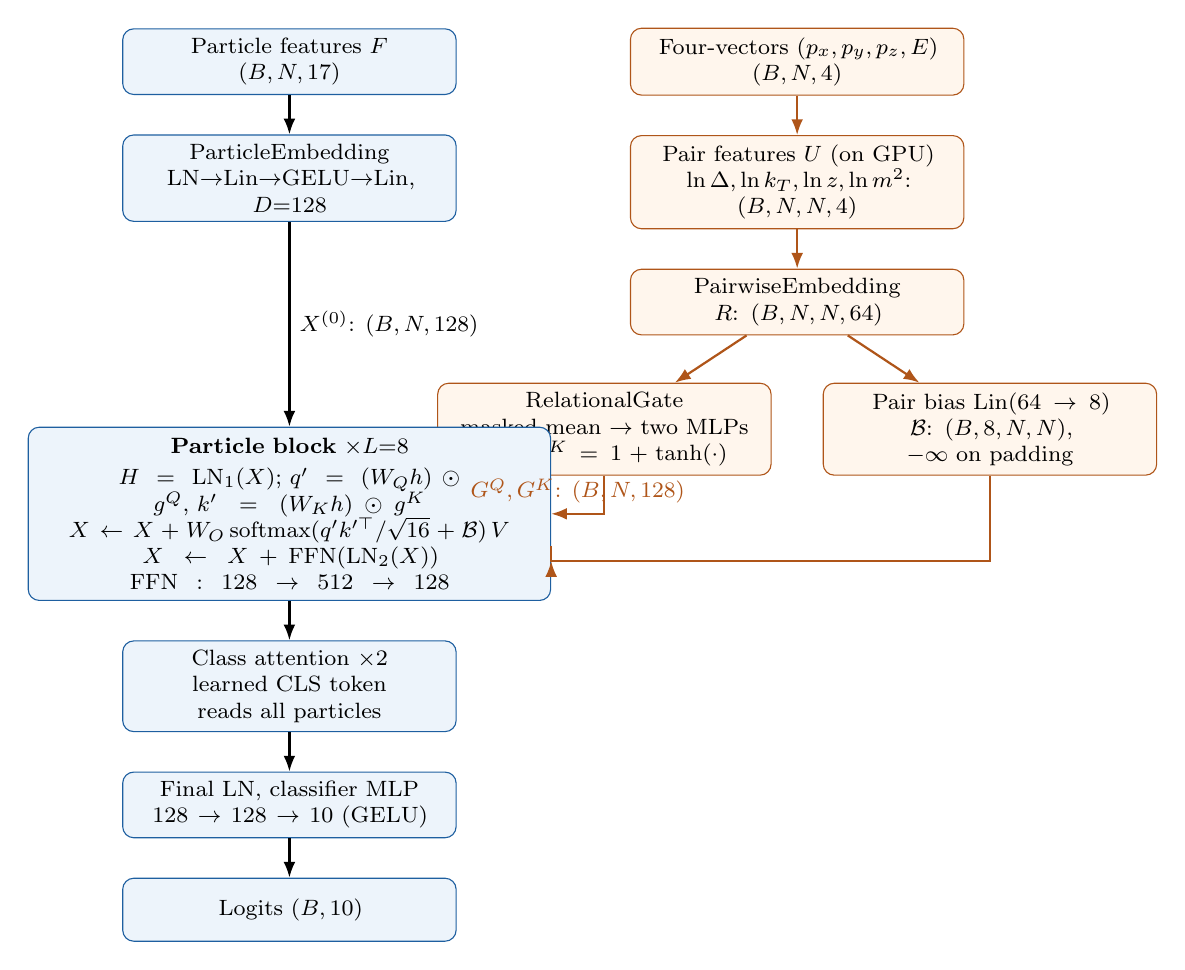
\begin{tikzpicture}[
  node distance=5mm and 8mm,
  every node/.style={font=\footnotesize},
  st/.style={draw,rounded corners,align=center,minimum height=8mm,text width=40mm,fill=softblue,draw=particleblue},
  pt/.style={draw,rounded corners,align=center,minimum height=8mm,text width=40mm,fill=orange!7,draw=pairorange},
  ar/.style={-{Latex[length=2mm]},thick},
  par/.style={-{Latex[length=2mm]},thick,pairorange}]
 \node[st] (f) {Particle features $F$\\$(B,N,17)$};
 \node[st,below=of f] (pe) {ParticleEmbedding\\LN$\to$Lin$\to$GELU$\to$Lin, $D{=}128$};
 \node[pt,right=22mm of f] (v) {Four-vectors $(p_x,p_y,p_z,E)$\\$(B,N,4)$};
 \node[pt,below=of v] (u) {Pair features $U$ (on GPU)\\$\ln\Delta,\ln k_T,\ln z,\ln m^2$: $(B,N,N,4)$};
 \node[pt,below=of u] (r) {PairwiseEmbedding\\$R$: $(B,N,N,64)$};
 \node[pt,below left=6mm and -18mm of r] (g) {RelationalGate\\masked mean $\to$ two MLPs\\$G^Q,G^K=1+\tanh(\cdot)$};
 \node[pt,below right=6mm and -18mm of r] (b) {Pair bias Lin$(64\to8)$\\$\mathcal B$: $(B,8,N,N)$, $-\infty$ on padding};
 \node[st,below=26mm of pe,text width=64mm,minimum height=22mm] (blk) {};
 \node[align=center,text width=62mm] at (blk) {\textbf{Particle block} $\times L{=}8$\\[2pt]
   $H=\LN_1(X)$;\ $q'=(W_Qh)\Had g^Q$, $k'=(W_Kh)\Had g^K$\\
   $X\leftarrow X+W_O\,\mathrm{softmax}(q'k'^\top/\sqrt{16}+\mathcal B)\,V$\\
   $X\leftarrow X+\FFN(\LN_2(X))$\\ $\FFN:128\to512\to128$};
 \node[st,below=of blk] (cls) {Class attention $\times2$\\learned CLS token reads all particles};
 \node[st,below=of cls] (head) {Final LN, classifier MLP\\$128\to128\to10$ (GELU)};
 \node[st,below=of head] (out) {Logits $(B,10)$};
 \draw[ar] (f)--(pe); \draw[ar] (pe)--node[right]{$X^{(0)}$: $(B,N,128)$}(blk);
 \draw[par] (v)--(u); \draw[par] (u)--(r); \draw[par] (r)--(g); \draw[par] (r)--(b);
 \draw[par] (g.south)|-node[pos=0.75,above]{$G^Q,G^K$: $(B,N,128)$}(blk.east);
 \draw[par] (b.south)|-([yshift=-6mm]blk.east)--([yshift=-6mm]blk.east);
 \draw[ar] (blk)--(cls); \draw[ar] (cls)--(head); \draw[ar] (head)--(out);
\end{tikzpicture}
\caption{GDS-ParT v2 as trained for the reported run (shared gates, pair bias, two CLS blocks).
In the code's default configuration the RelationalGate moves inside each particle block and
its neighbour aggregation is conditioned on the block's normalised particle state.
The pair embedding and the pair-bias projection are shared by all blocks.}
\label{fig:arch}
\end{figure}

\subsection{Configurations}
Every choice is a constructor argument of \code{GDSParTConfig} and a command-line flag of
\code{train_gds_part.py}. Table~\ref{tab:configs} lists the configurations that appear in the
results. Parameter counts were obtained by summing \code{p.numel()} over the instantiated model.

\begin{table}[ht]
\centering\small
\begin{tabular}{lcccc}
\toprule
 & v1 & v2 shared (reported) & v2 default & v2, no gates\\ \midrule
\code{gate_mode} & sigmoid & identity & identity & none\\
\code{per_layer_gate} & 0 & 0 & 1 & --\\
\code{pair_bias} & 0 & 1 & 1 & 1\\
\code{n_layers} & 6 & 8 & 8 & 8\\
\code{n_cls_layers} (0 = mean pool) & 0 & 2 & 2 & 2\\
Parameters & 1,280,684 & 2,074,420 & 2,488,116 & 2,024,756\\
\bottomrule
\end{tabular}
\caption{Model configurations. All use $D=128$, $H=8$ heads ($d=16$), FFN width 512,
$D_p=64$, dropout 0.1 and at most 128 particles per jet. The gates-only variant (v2 default without
pair bias) has 2,487,596 parameters.}
\label{tab:configs}
\end{table}

The following sections derive each box of Figure~\ref{fig:arch}: the input features
(Section~\ref{sec:inputs}), the two embeddings, attention with additive bias and with gates,
what the gates control, their expressivity and gradients, and the complete recurrence.

\section{Embeddings and the meaning of dual stream}
\subsection{Particle embedding}
For the column-vector description of particle $i$,
\begin{equation}\label{eq:particleembed}
 x_i^{(0)}=
 \Drop\!\left(W_2\GELU(W_1\LN_{17}(f_i)+b_1)+b_2\right),
\end{equation}
where $W_1\in\R^{D\times17}$ and $W_2\in\R^{D\times D}$.
This is \code{ParticleEmbedding}. Its weights are shared across particles.

The output is a learned description of one constituent. There is no
guarantee that coordinate 7 means charge or coordinate 83 means
displacement. A learned basis can mix several inputs and can change during
training. Raising the dimension to 128 is not adding 111 new measurements.

\subsection{Pair embedding}
Separately, \code{PairwiseEmbedding} computes
\begin{equation}\label{eq:pairembed}
 r_{ij}=W_4\GELU(W_3U_{ij}+b_3)+b_4,
\end{equation}
with $W_3\in\R^{D_p\times4}$, $W_4\in\R^{D_p\times D_p}$.
There is no LayerNorm or dropout inside this pair-embedding module.
With $D_p=64$, its parameter count is
$(4\cdot64+64)+(64^2+64)=4{,}480$.

\subsection{Why ``dual-stream''?}
There are \textbf{two representations with different index structure}:
\begin{align}
 \text{particle stream:}\quad &X^{(\ell)}\in\R^{B\times N\times D},\\
 \text{relation stream:}\quad &R\in\R^{B\times N\times N\times D_p}.
\end{align}
The first represents objects. The second represents relations between
objects. ``Dual'' does not refer to Q and K: ordinary attention already
has Q, K and V. Nor does it mean two independent jet classifiers.

\begin{figure}[ht]
\centering
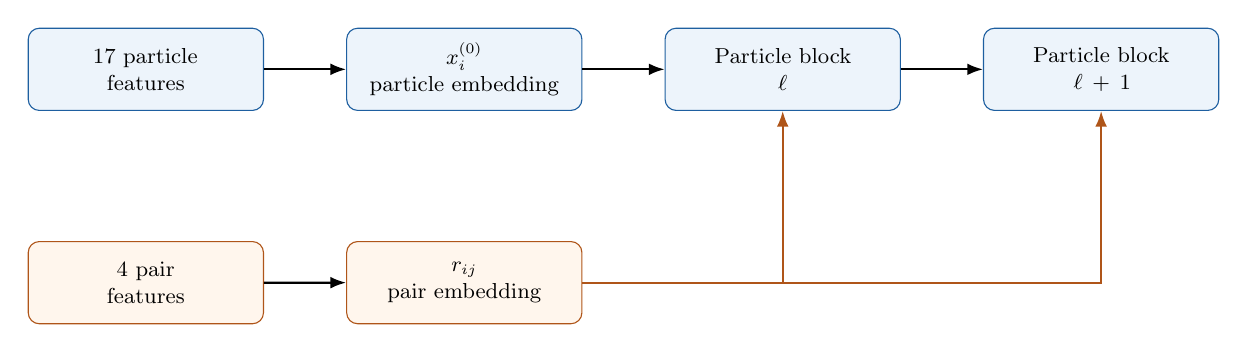
\begin{tikzpicture}[scale=0.87,transform shape]
 \node[pbox] (f) {17 particle\\features};
 \node[pbox,right=12mm of f] (x) {$x_i^{(0)}$\\particle embedding};
 \node[pbox,right=12mm of x] (b1) {Particle block\\$\ell$};
 \node[pbox,right=12mm of b1] (b2) {Particle block\\$\ell+1$};
 \node[pairbox,below=19mm of f] (u) {4 pair\\features};
 \node[pairbox,right=12mm of u] (r) {$r_{ij}$\\pair embedding};
 \draw[arrow] (f)--(x); \draw[arrow] (x)--(b1); \draw[arrow] (b1)--(b2);
 \draw[arrow] (u)--(r);
 \draw[arrow,pairorange] (r.east)-|(b1.south);
 \draw[arrow,pairorange] (r.east)--++(57mm,0)-|(b2.south);
\end{tikzpicture}
\caption{Two streams, fused inside attention. The relation tensor is reused;
the particle stream is updated by successive blocks.}
\end{figure}

In this implementation, $R$ is computed once per forward pass.
It is \textbf{not} a second recurrent transformer state updated after every
particle block. In per-layer gating, different blocks read the same $R$
through different learned, particle-state-conditioned summaries.

\subsection{How the streams meet}
The particle stream generates Q, K and V. The relation stream generates:
\begin{enumerate}
 \item query and key gates via per-particle summaries;
 \item optionally, an additive scalar bias for each head and pair.
\end{enumerate}
The first path is the GDS mechanism. The second is the ParT-style path.
They coexist in v2, so the trained v2 system is a hybrid rather than a
pure replacement of additive bias.

\begin{caution}
The original ParT also has particle and interaction embeddings. The name
``dual-stream'' does not establish a unique novelty by itself.
The specific architectural change here is \emph{using aggregated relations
to modulate Q and K channel by channel before their dot product}.
The exact MLPs and normalisation in this repository should not be attributed
unchanged to the published ParT implementation.
\end{caution}

\section{Self-attention, derived step by step}\label{sec:attn}
\subsection{Queries, keys and values}
Given a normalised particle vector $h_i\in\R^D$,
\begin{align}
 q_i&=W_Qh_i+b_Q,& k_i&=W_Kh_i+b_K,& v_i&=W_Vh_i+b_V.
\end{align}
``Query'', ``key'' and ``value'' are functional names:
the query and key determine the weight, while the value is the vector
being combined. These are learned projections, not manually selected
particle attributes.

For row-stored $X\in\R^{N\times D}$, this is
$Q=XW_Q^\top+\mathbf1 b_Q^\top$ and similarly for K and V.
We suppress the batch index when studying one jet.

\subsection{One attention head}
Within a head, each vector has $d$ channels. Its logits and weights are
\begin{align}
 S_{ij}&=\frac{q_i^\top k_j}{\sqrt d}+M_{ij},\\
 A_{ij}&=\softmax_j(S_{ij}),\\
 o_i&=\sum_j A_{ij}v_j.\label{eq:attnoutput}
\end{align}
The sum is over \emph{key} particles $j$ for each fixed query particle $i$.
Without training dropout, $o_i$ is a convex combination of the head's
value vectors. The output projection and residual addition afterwards
need not be convex combinations.

\begin{example}[Complete one-head calculation]
Take $q=(1,0)^\top$, $k_1=(1,0)^\top$, $k_2=(0,1)^\top$, with $d=2$.
Then the logits are $(1/\sqrt2,0)$ and the weights are approximately
$(0.6698,0.3302)$.
If $v_1=(2,0)^\top$ and $v_2=(0,4)^\top$, the output is
\[
 o=0.6698\begin{bmatrix}2\\0\end{bmatrix}
   +0.3302\begin{bmatrix}0\\4\end{bmatrix}
   \simeq\begin{bmatrix}1.3395\\1.3210\end{bmatrix}.
\]
The value vectors were not compared to decide the weights. Q and K
performed that comparison; V supplied the message.
\end{example}

\subsection{Why divide by the square root?}
Suppose the entries of q and k are independent, zero-mean and unit-variance,
with independent products across channels. Then
\[
 \Var\left(\sum_{c=1}^{d}q_ck_c\right)=d.
\]
Dividing by $\sqrt d$ gives variance 1. This is an initial scale argument,
not an exact description of trained, correlated features. It helps avoid
extreme softmax saturation at initialisation.

\subsection{Multiple heads and the output projection}
Split $D=128$ into $H=8$ groups of $d=16$ channels. Each head computes
its own $A^{(h)}$ and $O^{(h)}$:
\[
 O_{\rm cat}=[O^{(1)}\mid\cdots\mid O^{(H)}]\in\R^{N\times D},
 \qquad Y=O_{\rm cat}W_O^\top+\mathbf1b_O^\top.
\]
Heads allow distinct learned comparisons. Describing one as an ``angle
head'' requires evidence; architecture alone does not impose that role.

\subsection{Why particle order does not matter}
Let $P$ be a permutation matrix that reorders particles. With no
position-index embeddings, reordering $X$ to $PX$ gives
$Q\mapsto PQ$, $K\mapsto PK$, $V\mapsto PV$.
Thus
\[
 S\mapsto PSP^\top,\qquad
 A\mapsto PAP^\top,\qquad
 AV\mapsto PAV.
\]
The output reorders with the input: this is permutation
\emph{equivariance}. A symmetric pooling operation or a CLS summary then
gives permutation \emph{invariance} for the jet prediction.

\section{ParT-style attention: an additive relation term}
\subsection{The defining interaction mechanism}
ParT injects interaction features into attention logits.
Writing the learned interaction encoder abstractly as $\psi$:
\begin{equation}\label{eq:part}
 A^{(h)}=\softmax_{\rm row}
 \left(\frac{Q^{(h)}K^{(h)\top}}{\sqrt d}
       +\psi(U)^{(h)}+M\right).
\end{equation}
In this repository's local bias path,
\[
 \mathcal B_{ij}=W_{\rm bias}r_{ij}+b_{\rm bias}\in\R^H.
\]
There are $HD_p+H=520$ parameters in this last projection for $D_p=64,H=8$.
That count describes \emph{this projection}, not the complete original
ParT interaction encoder.

\subsection{An additive logit bias is a multiplicative unnormalised weight}
For valid keys, write the content score as $C_{ij}=q_i^\top k_j/\sqrt d$.
Then
\[
 A_{ij}=
 \frac{e^{C_{ij}}e^{\mathcal B_{ij}}}
 {\sum_t e^{C_{it}}e^{\mathcal B_{it}}}.
\]
The relation term acts like a learned factor on content-based weights.
Relative odds obey
\[
 \log\frac{A_{ij}}{A_{ik}}
 =C_{ij}-C_{ik}+\mathcal B_{ij}-\mathcal B_{ik}.
\]
It can change a pair's score even when its content dot product is zero.

\subsection{What ``pair-specific'' does and does not mean}
The bias reads the specific $U_{ij}$ rather than first averaging over
neighbours. However, it is not an arbitrary free $N\times N$ table.
The same network is applied to every pair, so equal pair features produce
equal biases. The symmetric pair features used here give symmetric biases.
Row softmax and the query--key projections can still produce asymmetric
attention weights.

The bias is independent of the current hidden particle state when $U$ is
held fixed. That does not mean it is independent of the event's physics,
or that it cannot affect particle representations: its changed weights
modify Equation~\eqref{eq:attnoutput} and therefore the next hidden states.

\section{GDS gates: the full construction}
\subsection{From pair vectors to one summary per particle}
The pair row for particle $i$ is $r_{i1},\ldots,r_{iN}$.
To create a particle-sized gate, the model reduces the neighbour index.

\subsubsection{Shared, masked-mean mode}
For one jet with $n=\sum_jm_j>0$:
\begin{equation}\label{eq:meansummary}
 s_i=\frac{\sum_jm_jr_{ij}}{n}\in\R^{D_p}.
\end{equation}
One \code{RelationalGate} computes a query/key gate pair reused in all
particle blocks. ``Shared'' means the \emph{same gate vector for that
particle across layers}, not one scalar or one vector for the entire jet.
Different particles generally get different gates.

\subsubsection{Per-layer, conditioned mode}
Block $\ell$ takes $h_i^{(\ell)}=\LN_1^{(\ell)}(x_i^{(\ell)})$ and computes
\begin{align}
 c_i^{(\ell)}&=W_{\rm ctx}^{(\ell)}h_i^{(\ell)}+b_{\rm ctx}^{(\ell)}
                         \in\R^{D_p},\\
 e_{ij}^{(\ell)}&=\frac{r_{ij}^\top c_i^{(\ell)}}{\sqrt{D_p}}+M_{ij},\\
 \alpha_{ij}^{(\ell)}&=\softmax_j(e_{ij}^{(\ell)}),\\
 s_i^{(\ell)}&=\sum_j\alpha_{ij}^{(\ell)}r_{ij}.
\end{align}
This is a small attention-like read of the relation row, distinct from
the main particle attention. Each block has its own context projection
and gate MLPs, but all blocks read the same pair tensor $R$.

\subsubsection{The diagonal is included in the actual aggregation}
The raw self-pair input $U_{ii}$ is zero. Nevertheless,
\[
 r_{ii}=W_4\GELU(b_3)+b_4
\]
need not be zero because the pair MLP has biases.
The gate masks exclude padded neighbours, not $j=i$.
Consequently the sums above include the self-pair relation.
This distinction matters when reproducing the implementation.

\subsection{Separate query and key gate MLPs}
For $a\in\{Q,K\}$, let
\begin{align}
 z_i^a&=W_2^a\GELU(W_1^a s_i+b_1^a)+b_2^a,\\
 g_i^a&=\mathbf1+\tanh(z_i^a)\in(0,2)^D.\label{eq:gate}
\end{align}
The two MLPs have separate parameters. In shared mode their combined
parameter count is
\[
 2[(D_pD+D)+(D^2+D)]=49{,}664.
\]
Conditioning adds $D_pD+D_p=8{,}256$ parameters per block, making
57,920 per conditioned gate module.

\subsection{Identity initialisation}
For \code{gate_mode="identity"}, the final affine weights and biases
$W_2^a,b_2^a$ are zero initially. Therefore $z_i^a=0$ and $g_i^a=1$
for every particle and channel.

This makes the \emph{gate path} an identity at initialisation.
With pair bias enabled, attention is still bias-augmented, not plain
attention. In sigmoid mode the last layer is normally random, so gates
are \emph{not guaranteed to be exactly 0.5}. The value 0.5 applies only
when the sigmoid input is zero.

Zero-initialisation does not permanently freeze the gates.
Since $\tanh'(0)=1$, the final gate layer can receive gradients immediately.
At the first step, gradients through $W_2^a=0$ to its earlier gate layers
vanish along that path; those earlier layers can receive gate-path gradients
once $W_2^a$ changes.

\subsection{Applying the gates}
Before splitting into heads, the code performs
\begin{equation}
 q'_i=q_i\Had g_i^Q,\qquad k'_i=k_i\Had g_i^K,\qquad v'_i=v_i.
\end{equation}
The complete v2 attention logits are
\begin{equation}\label{eq:gds}
 S^{(h)}_{ij}=
 \frac1{\sqrt d}\sum_{c\in h}
 q_{ic}g^Q_{ic}\,k_{jc}g^K_{jc}
 +\mathcal B^{(h)}_{ij}+M_{ij}.
\end{equation}
The gates operate on learned Q/K coordinates, not directly on the 17 raw
features. A gate near zero suppresses one coordinate in this comparison;
it does not delete the particle or erase its residual state.

\section{What query gates and key gates actually control}
\subsection{A query gate changes one query's comparisons}
Hold all other forward-pass quantities fixed. Changing $g^Q_i$ changes
row $i$ of the content score matrix:
\[
 \frac{\partial S_{ij}}{\partial g^Q_{ic}}
 =\frac{q_{ic}k_{jc}g^K_{jc}}{\sqrt d}.
\]
The sign depends on the signed feature product. Increasing the gate can
increase or decrease a score.
The gate changes which combinations of features matter when particle $i$
compares itself with the keys.

\subsection{A key gate changes how one key is matched}
Similarly,
\[
 \frac{\partial S_{ij}}{\partial g^K_{jc}}
 =\frac{q_{ic}g^Q_{ic}k_{jc}}{\sqrt d}.
\]
Changing key gate $g^K_j$ directly changes content logits in column $j$.
After row softmax, weights for \emph{all} keys in affected rows can change
because the normalising denominator changes.

\begin{example}[A larger key can get less attention]
Use scalar $q=1$, $k_1=-1$, $k_2=0$, with no bias and $d=1$.
Initially, logits are $(-1,0)$ and the weight on key 1 is approximately
0.269. Doubling key 1 with $g^K_1=2$ changes the logits to $(-2,0)$,
and its weight becomes approximately 0.119.
\end{example}

\begin{takeaway}
Query gating changes how a particle searches.
Key gating changes how a particle can be matched.
Neither means ``more gate equals more attention'' in general.
\end{takeaway}

\subsection{When the temperature analogy is valid}
If a query gate multiplies every channel of a head by the same positive
scalar $a$, and there is no varying additive bias, then
\[
 \softmax(aC_{i,:})=\softmax(C_{i,:}/T),\qquad T=1/a.
\]
That special case is temperature scaling. General channel-wise gates
can change the \emph{ordering} of scores, and adding a fixed nonuniform
pair bias means $\softmax(aC+\mathcal B)$ is not a simple temperature
rescaling of $\softmax(C+\mathcal B)$.

Means such as $D^{-1}\sum_cg^Q_{ic}$ discard the signed Q/K products.
They cannot establish which partners receive more attention. To show
core-to-periphery transfer, one would need changes in the actual
attention weights grouped by particle locations, and preferably changes
in weighted value contributions or downstream outputs as well.

\subsection{Why separate Q and K gates?}
Queries and keys have different learned projections and different roles.
Separate gates let a particle use different channel weights when it is a
query and when it is a key. This permits asymmetric matching even when
pair inputs are symmetric.

There is also a scale ambiguity: multiplying every $g^Q_{ic}$ in a channel
by $a$ and dividing every $g^K_{jc}$ by $a$ leaves the content scores
unchanged where the transformed gates remain allowed. Learned projection
weights add more reparameterisation freedom. Gate magnitudes are therefore
not uniquely identifiable measures of physical importance.

\subsection{Why is V not gated here?}
The current design modulates matching and leaves $v_j=W_Vh_j+b_V$
unchanged directly. Attention still changes the combined message by
changing its coefficients. Gating V is a possible alternative architecture,
not an operation proven unnecessary by this implementation.

\section{Expressivity: additive bias versus multiplicative gates}
\subsection{A context-dependent diagonal bilinear form}
Within one head,
\begin{equation}
 q_i'{}^\top k_j'
 =q_i^\top\diag(g_i^Q\Had g_j^K)k_j.
\end{equation}
The diagonal entries are positive and depend on the input through relations.
This is a useful \emph{comparison-weighting} interpretation.
It is not generally a distance metric on particles: Q and K differ, and
the diagonal matrix depends on both indices. Symmetry and triangle
inequalities need not hold.

\subsection{The factorised structure}
For channel $c$, the array of gate multipliers is
\[
 T_{ijc}=g^Q_{ic}g^K_{jc},\qquad
 T_{:,:,c}=g^Q_{:,c}(g^K_{:,c})^\top.
\]
It has rank at most 1. But the full content logits are a \emph{sum} across
channels:
\[
 S_{\rm content}=\frac1{\sqrt d}(Q\Had G^Q)(K\Had G^K)^\top,
 \qquad \rank(S_{\rm content})\le d.
\]
Plain content attention has the same rank bound. Gating changes the
input-dependent vectors that enter the factorisation; it does not remove
the factorisation.

\subsection{What is gained and what is lost by summarising relations?}
The summary $s_i\in\R^{D_p}$ compresses the entire row of relation vectors.
This is permutation-invariant in the neighbour dimension, but it can lose
information about which partner produced which relation.
The bias path directly reads $r_{ij}$ for each pair and can express a
nonlinear pair table whose rank exceeds $d$.

It would be too strong to say gates cannot distinguish individual partners.
The content keys still distinguish partners, and multiple channels
contribute. The precise limitation is a compressed context and a
factorised content-score parameterisation, compared with direct
pair-feature access in the additive bias.

\subsection{A numerical comparison}
Reuse $q=(1,0)$, $k_1=(1,0)$ and $k_2=(0,1)$ from Section~\ref{sec:attn}.
Bias $(0,1)$ gives logits $(0.7071,1)$ and weights approximately
$(0.4273,0.5727)$: the bias can favour the key orthogonal to the query.

With no bias, set $g^Q=(0.5,1)$ and both key gates to 1.
The logits become $(0.3536,0)$ and weights approximately
$(0.5875,0.4125)$. The gate reduces the preference for key 1, but cannot
make the originally zero second query channel nonzero in this example.
In a trained network, the upstream projections also change and can
represent information in other channels.

\subsection{Controlled baselines}
Four local comparisons answer different questions:
\begin{center}
\begin{tabular}{lll}
\toprule Model & Gates & Pair bias\\ \midrule
Plain-style baseline & off & off\\
ParT-style baseline & off & on\\
Gates-only model & on & off\\
Hybrid GDS-ParT & on & on\\
\bottomrule
\end{tabular}
\end{center}
For a fair ablation, hold data, preprocessing, optimisation budget and
evaluation samples fixed. Differences in depth, pooling, parameter count,
EMA or label smoothing can confound an apparent architectural gain.
The v1-to-v2 change includes several such changes, so its accuracy increase
cannot be attributed solely to adding the bias.

\section{Backpropagation through attention and gates}
\subsection{From output messages to attention scores}
For a head, let $o_i=\sum_j A_{ij}v_j$ and
$\delta_i=\partial\mathcal L/\partial o_i$. Then
\[
 \frac{\partial\mathcal L}{\partial A_{ij}}=\delta_i^\top v_j.
\]
Using the softmax Jacobian,
\begin{equation}\label{eq:scoregrad}
 \frac{\partial\mathcal L}{\partial S_{ij}}
 =A_{ij}\,\delta_i^\top(v_j-o_i).
\end{equation}
A key's value is compared with the current average message in the
direction relevant to the loss. This explains why an attention weight
alone is not the same as a feature's importance.

\subsection{Gradients to Q, K, gates and bias}
Write $E_{ij}=\partial\mathcal L/\partial S_{ij}$. For one head:
\begin{align}
 \frac{\partial\mathcal L}{\partial g^Q_{ic}}
 &=\sum_j E_{ij}\frac{q_{ic}k_{jc}g^K_{jc}}{\sqrt d},\\
 \frac{\partial\mathcal L}{\partial g^K_{jc}}
 &=\sum_i E_{ij}\frac{k_{jc}q_{ic}g^Q_{ic}}{\sqrt d},\\
 \frac{\partial\mathcal L}{\partial q_{ic}}
 &=\sum_j E_{ij}\frac{g^Q_{ic}k_{jc}g^K_{jc}}{\sqrt d},\\
 \frac{\partial\mathcal L}{\partial\mathcal B_{ij}}
 &=E_{ij}.
\end{align}
For $g=1+\tanh z$:
\[
 \frac{\partial\mathcal L}{\partial z}
 =\frac{\partial\mathcal L}{\partial g}\Had(1-\tanh^2z).
\]
Saturated gates near 0 or 2 can have small derivatives. Positive gates
cannot flip the sign of a single Q or K coordinate, but they can change
the sign of a total score by reweighting its positive and negative terms.

\subsection{Gradient through a shared summary}
For the masked mean in Equation~\eqref{eq:meansummary}, its direct
Jacobian is
\[
 \frac{\partial s_{ic}}{\partial r_{ijc'}}=
 \frac{m_j}{n}\delta_{cc'}.
\]
The shared gate receives gradient contributions from every block that uses
it. Pair embeddings receive gradients from both gate and bias paths when
both are enabled.

\subsection{Gradient through the conditioned summary}
Suppress $i,\ell$ and write $s=\sum_j\alpha_jr_j$,
$\alpha=\softmax(e)$. Then
\[
 \frac{\partial s}{\partial e_j}=\alpha_j(r_j-s).
\]
For $u=\partial\mathcal L/\partial s$ and
$e_j=r_j^\top c/\sqrt{D_p}$:
\begin{align}
 \frac{\partial\mathcal L}{\partial c}
 &=\frac1{\sqrt{D_p}}\sum_j
       \alpha_j\big[u^\top(r_j-s)\big]r_j,\\
 \frac{\partial\mathcal L}{\partial r_j}
 &=\alpha_j u+
   \frac{\alpha_j\,u^\top(r_j-s)}{\sqrt{D_p}}c .
\end{align}
These expressions describe the summary path; other uses of $R$ add further
gradient contributions. The context projection then propagates gradients
back into the current particle state $h_i$.

\section{The complete GDS-ParT forward pass}
\subsection{Particle-block recurrence}
For $\ell=0,\ldots,L-1$:
\begin{align}
 H^{(\ell)}&=\LN_1^{(\ell)}(X^{(\ell)}),\\
 (G_Q^{(\ell)},G_K^{(\ell)})&=
 \begin{cases}
 (G_Q,G_K),&\text{shared mode},\\
 \operatorname{Gate}_{\ell}(R,H^{(\ell)},m),&\text{conditioned mode},
 \end{cases}\\
 \widetilde X^{(\ell)}
 &=X^{(\ell)}+
 \operatorname{GatedAttention}_{\ell}
 (H^{(\ell)},G_Q^{(\ell)},G_K^{(\ell)},\mathcal B,M),\\
 X^{(\ell+1)}
 &=\widetilde X^{(\ell)}
   +\FFN_\ell(\LN_2^{(\ell)}(\widetilde X^{(\ell)})).
\end{align}
Each block has separate Q/K/V/output projections, normalisations and FFN.
The pair embedding and pair-bias projection are shared across blocks.

\subsection{Class-attention pooling}
Start with a learned vector $c^{(0)}\in\R^D$.
For a class-attention block, concatenate it with the final particles:
\[
 Z=\LN([c;X^{(L)}]).
\]
Only the first row is used as the query. All valid rows, including the
CLS row, supply keys and values. The code updates
\begin{align}
 \widetilde c&=c+\operatorname{MHA}(Z_{\rm CLS},Z,Z),\\
 c_{\rm next}&=\widetilde c+\FFN(\LN(\widetilde c)).
\end{align}
Two such blocks update the CLS token; the particle states remain fixed.
These are ordinary class-attention modules, not Q/K-gated particle blocks.
They do not receive the pairwise bias.

In the older mean-pooling option, the model instead normalises the final
particle states and takes their masked mean. That is a different pooling
mechanism, not simply a missing CLS token with otherwise identical behaviour.

\subsection{Classifier}
After class attention, let $z=\LN_{\rm final}(c)$. The classifier is
\[
 \ell=W_{\rm out}\Drop(\GELU(W_{\rm hid}z+b_{\rm hid}))+b_{\rm out}
       \in\R^{10}.
\]
The forward method returns these logits, not softmax probabilities.
Training cross-entropy consumes logits directly; evaluation applies
softmax when probabilities or ROC scores are required.

\subsection{Permutation properties with both streams}
Reordering particles must also reorder both particle axes of $R$ and the
mask. Shared and conditioned summaries reorder with the particles, so the
gates do as well. The gated score matrix and pair bias transform as
$S\mapsto PSP^\top$. Every particle block remains equivariant.
CLS attention or masked-mean pooling produces an invariant jet result.
This argument describes evaluation; stochastic dropout must be permuted
consistently to demand exact equality in a particular training draw.

\section{Training}\label{sec:training}
\subsection{Objective and label smoothing}
For a true class $y$, the smoothed target in the reported v2 recipe is
\[
 t_k=(1-\varepsilon_{\rm LS})\,\mathbf1[k=y]
           +\frac{\varepsilon_{\rm LS}}{10},\qquad
 \varepsilon_{\rm LS}=0.1.
\]
Thus the true-class target is 0.91 and each other class has target 0.01.
The loss over a batch is
\[
 \mathcal L_{\rm CE}
 =-\frac1B\sum_{b=1}^{B}\sum_{k=1}^{10}t_{bk}\ln p_{bk}.
\]
Label smoothing discourages extreme confidence. Whether it improves
accuracy or calibration in a given setting must be measured.

\subsection{AdamW}
Let $g_t$ be the gradient at step $t$:
\begin{align}
 m_t&=\beta_1m_{t-1}+(1-\beta_1)g_t,\\
 v_t&=\beta_2v_{t-1}+(1-\beta_2)g_t^2,\\
 \widehat m_t&=m_t/(1-\beta_1^t),\qquad
 \widehat v_t=v_t/(1-\beta_2^t),\\
 \theta_{t+1}
 &=(1-\eta_t\lambda)\theta_t
 -\eta_t\frac{\widehat m_t}{\sqrt{\widehat v_t}+\epsilon_{\rm opt}} .
\end{align}
Squares, roots and division are element-wise. The moment vectors estimate
gradient direction and squared size. AdamW's weight decay is decoupled
from the adaptive gradient update.

\subsection{Schedule, clipping and EMA}
The training recipe uses a linear warm-up, followed by cosine decay.
Writing total steps $T$ and warm-up steps $T_w$:
\[
 \eta_t=\eta_{\max}
 \begin{cases}
 t/\max(1,T_w),&t<T_w,\\
 \tfrac12[1+\cos(\pi(t-T_w)/\max(1,T-T_w))],&t\ge T_w.
 \end{cases}
\]
The code clamps the cosine progress to 1. Gradient clipping with threshold
$C$ replaces $g$ by $g\min(1,C/\|g\|_2)$.

An exponential moving average maintains
$\bar\theta_t=\rho\bar\theta_{t-1}+(1-\rho)\theta_t$ after initialisation.
The trainer's default is $\rho=0.999$; both 10M-jet v2 runs (10 and 20 epochs) used
$\rho=0.9999$, as recorded in their saved arguments. EMA weights can lag far behind rapidly
changing early training, so very short-run EMA comparisons need care.

\subsection{Micro-batches, precision and checkpointing}
A batch of $B$ jets can be split into pieces. For piece $s$ of size $B_s$,
backpropagating $(B_s/B)\mathcal L_s$ and accumulating gradients before
one optimiser step reproduces the full-batch mean-loss gradient, apart
from stochastic and floating-point effects.

Mixed precision uses suitable lower-precision operations on CUDA while
retaining important calculations in higher precision.
Loss scaling reduces FP16 underflow. The CPU path in this trainer does
not enable that CUDA autocast.

Activation checkpointing recomputes block internals during backward to
save stored activations. It does not save the model to disk.
Disk checkpoints instead store model weights, raw/EMA state, optimiser,
scheduler and progress needed to resume the run.

\subsection{Training recipe of the reported run}
Table~\ref{tab:hyper} lists the settings recorded in \code{results.json} of the reported run.
The weight decay applies to all parameters (one parameter group).
\begin{table}[ht]
\centering\small
\begin{tabular}{p{50mm}p{95mm}}
\toprule Setting & Value\\ \midrule
Training jets / epochs & 10,000,000 / 10 \\
Batch size / steps per epoch / total steps & 512 / 19,532 / 195,320\\
Optimiser & AdamW, $\eta_{\max}=10^{-3}$, $\lambda=0.01$, $\beta=(0.9,0.999)$, $\epsilon=10^{-8}$\\
Schedule & linear warm-up over 5\% (9,766 steps), cosine decay to 0\\
Gradient clipping & global $\ell_2$ norm 1.0\\
Label smoothing & 0.1\\
EMA decay $\rho$ & 0.9999 (evaluation and checkpoints use EMA weights)\\
Dropout & 0.1 (embedding, attention, FFN, classifier)\\
Precision & CUDA autocast float16 with gradient scaling\\
Micro-batching & $BN^2\le2\times10^6$ per forward pass\\
Seed & 0\\
\bottomrule
\end{tabular}
\caption{Optimisation settings for the reported 10M-jet run.}
\label{tab:hyper}
\end{table}

With $\rho=0.9999$ the EMA averages over an effective horizon of $1/(1-\rho)=10^4$ steps, about half
an epoch here. The ablations of Section~\ref{sec:exp} show why this horizon must be short compared
with the run: with $\rho=0.999$ and only 1,172 steps, the weights after the first step still carry
a weight of $0.999^{1171}\approx0.31$ in the EMA at the end of training.


%====================================================================
\section{Evaluation metrics}\label{sec:metrics}
%====================================================================
All metrics are computed by \code{compute_jet_tagging_metrics} in \code{train_gds_part.py}
from the softmax scores $p_{bk}$ of the evaluation weights (the EMA copy when EMA is on), and
follow Section~2 of the ParT paper~[\ref{ref:part}].

\paragraph{Accuracy.} With $\hat y_b=\arg\max_k p_{bk}$,
\begin{equation}
 \mathrm{Acc}=\frac1{n}\sum_{b=1}^{n}\mathbf 1[\hat y_b=y_b].
\end{equation}
Per-class accuracy is the diagonal of the row-normalised confusion matrix $C_{kk'}=\#\{b:y_b=k,\hat y_b=k'\}$.

\paragraph{Macro one-vs-one AUC.} For an ordered class pair $(j,k)$, restrict to jets of class
$j$ or $k$ and compute the ROC AUC of the score $p_{bj}$ for separating $j$ from $k$:
\begin{equation}
 \mathrm{AUC}(j\,|\,k)=\Pr\big(p_{b j}>p_{b' j}\,\big|\,y_b=j,\ y_{b'}=k\big)
   +\tfrac12\Pr\big(p_{bj}=p_{b'j}\big).
\end{equation}
The reported value is the Hand--Till average over the $K(K-1)/2=45$ unordered pairs,
\begin{equation}
 \mathrm{AUC}_{\rm macro}^{\rm ovo}=\frac{2}{K(K-1)}\sum_{j<k}
 \frac{\mathrm{AUC}(j\,|\,k)+\mathrm{AUC}(k\,|\,j)}{2},
\end{equation}
as implemented by \code{sklearn.metrics.roc_auc_score(..., multi_class="ovo", average="macro")}.

\paragraph{Background rejection at fixed signal efficiency.} For each signal class $S$ against
QCD ($B$), restrict to jets of the two classes and form the two-class discriminant
\begin{equation}
 \mathcal D_{S}=\frac{p_S}{p_S+p_B+10^{-12}} .
\end{equation}
Scanning a threshold on $\mathcal D_S$ gives the ROC curve $(\epsilon_B,\epsilon_S)$ with
$\epsilon_S$ the signal efficiency (true-positive rate) and $\epsilon_B$ the QCD mistag rate
(false-positive rate). The rejection at signal efficiency $X\%$ is
\begin{equation}
 \mathrm{Rej}_{X\%}=\frac1{\epsilon_B(\epsilon_S=X\%)} ,
\end{equation}
with $\epsilon_B$ obtained by linear interpolation of the ROC curve. As in the paper,
$X=50$ for all signals except $H\to\ell\nu qq'$ ($X=99$) and $t\to b\ell\nu$ ($X=99.5$), whose
leptons make them easy to separate.

\paragraph{Statistical resolution.} With $n$ test jets, the binomial standard error of the
accuracy is $\sqrt{\mathrm{Acc}(1-\mathrm{Acc})/n}\approx3.6\times10^{-4}$ for $n=10^6$.
Rejections are far less precise. A rejection of $R$ measured on $n_B$ QCD jets is set by about
$n_B/R$ surviving background jets, with a relative Poisson uncertainty of roughly
$\sqrt{R/n_B}$. On the $10^5$ QCD jets of the test subset, $\mathrm{Rej}=10{,}000$ rests on about
ten jets ($\approx30\%$ uncertainty), whereas $\mathrm{Rej}\approx100$ rests on about a thousand.


%====================================================================
\section{Results}\label{sec:results}
%====================================================================
All numbers in this section are read from files committed to the repository:
\code{results/v2_shared_10M_10ep/results.json} and \code{RESULTS.md},
\code{results/jetclass_10M/results.json} (v1), \code{results/part_official_validation.json},
\code{checkpoints/v2_shared_10M_20ep/events.jsonl}, and the ablation summaries in
\code{results/ablation_summaries/}. Published reference numbers are taken from Tables~1 and~3 of the ParT
paper~[\ref{ref:part}], as tabulated by \code{make_report.py}.

\subsection{Evaluation sets}
Training used 10 million jets from the official JetClass training split (19,532 batches of 512
per epoch). Validation used a balanced subset of one million jets and testing a
separate balanced subset of one million jets (100,000 per class) from the official 20M-jet test
split. The checkpoint with the best validation accuracy is used for testing; for the reported run
this is the last epoch.

\subsection{Validating the pipeline with the official ParT}\label{sec:validation}
Before trusting any comparison, \code{validate_pipeline.py} evaluates the official pretrained
ParT checkpoint (trained on 100M jets) on our cached test data, using our preprocessing (after
permuting the feature order to the official one) and our metric code, on 200,000 test jets.

\begin{table}[ht]
\centering\small
\begin{tabular}{lcc}
\toprule & Accuracy & Macro AUC\\ \midrule
Official ParT, our pipeline (200k jets) & 0.8612 & 0.98771\\
Official ParT, paper (20M jets) & 0.861 & 0.9877\\
\bottomrule
\end{tabular}
\caption{Pipeline check. Accuracy and AUC agree to the quoted precision, so the 17 features,
the 4 pair features, the labels and the metric definitions match the reference.}
\label{tab:validation}
\end{table}
The rejections from this check scatter widely around the paper values (for example 4,997 against
10,638 for $H\to b\bar b$ and an infinite value for $t\to bqq'$) because only about 20,000 QCD
jets are available: a rejection of 9,993 corresponds to two surviving jets. This illustrates the
statistical caveat of Section~\ref{sec:metrics}.

\subsection{Main result: v2 shared, 10 million jets, 10 epochs}
\begin{table}[ht]
\centering\footnotesize
\setlength{\tabcolsep}{2.4pt}
\begin{tabular}{lrrcccccccccc}
\toprule
Model & Params & Acc & AUC & \multicolumn{9}{c}{Rejection (Rej$_{50\%}$ unless noted)}\\
\cmidrule(lr){5-13}
 & & & & $Hbb$ & $Hcc$ & $Hgg$ & $H4q$ & $Hqql$\textsuperscript{a} & $Tbqq$ & $Tbl$\textsuperscript{b} & $Wqq$ & $Zqq$\\ \midrule
ParticleNet (10M)\textsuperscript{c} & 370k & 0.837 & 0.9837 & 5848 & 2070 & 96 & 770 & 2350 & 5495 & 6803 & 307 & 253\\
ParT (10M)\textsuperscript{c} & 2.14M & 0.850 & 0.9860 & 8734 & 3040 & 110 & 1274 & 3257 & 12579 & 8969 & 431 & 324\\
ParT (100M)\textsuperscript{c} & 2.14M & 0.861 & 0.9877 & 10638 & 4149 & 123 & 1864 & 5479 & 32787 & 15873 & 543 & 402\\ \midrule
GDS-ParT v1 (10M) & 1.28M & 0.8272 & 0.9824 & 6667 & 1695 & 102 & 709 & 1449 & 4762 & 5263 & 285 & 254\\
GDS-ParT v2 (10M) & 2.07M & \textbf{0.8484} & \textbf{0.9853} & 7143 & 2259 & 104 & 1250 & 1923 & 10000 & 3846 & 328 & 264\\
\bottomrule
\end{tabular}
\caption{Test results. \textsuperscript{a}Rej$_{99\%}$. \textsuperscript{b}Rej$_{99.5\%}$.
\textsuperscript{c}Published values on the full 20M test set; GDS-ParT rows use the
one-million-jet subset and their training budget is much smaller (see text).}
\label{tab:main}
\end{table}

GDS-ParT v2 reaches a test accuracy of 0.848428 and a macro AUC of 0.985333 (test cross-entropy
0.5167), against 0.850 and 0.9860 for ParT trained on the same number of jets. The differences,
$-0.0016$ in accuracy and $-0.0007$ in AUC, are small, but the comparison is not controlled:
\begin{itemize}
 \item ParT was trained for 1M iterations of batch 512 (about 512M jets seen) with
   Lookahead(RAdam); this run saw 100M jets (10 epochs) with AdamW and a cosine schedule on a 6\,GB
   laptop GPU, at roughly 70--85 minutes per epoch.
 \item Our test subset is 1M rather than 20M jets.
 \item The model is a hybrid that also uses an additive pair bias.
\end{itemize}
Rejections are lower than ParT (10M) for most signals, markedly so for $H\to\ell\nu qq'$ (1,923
against 3,257) and $t\to b\ell\nu$ (3,846 against 8,969), and comparable for $H\to4q$ (1,250
against 1,274). The highest values rest on 10--30 surviving QCD jets, so only differences of
a factor of order two are meaningful.

\paragraph{Per-class behaviour.} Table~\ref{tab:perclass} lists per-class test accuracy. The
dominant confusions in the test confusion matrix are $Z\to q\bar q$ predicted as $W\to qq'$
(16,847 of 100,000) and the reverse (12,351), $H\to gg$ against $H\to 4q$ (8,231 and 7,995),
and QCD predicted as $H\to gg$ (7,997). The two leptonic classes $H\to\ell\nu qq'$ and
$t\to b\ell\nu$ are confused mainly with each other (1,079 and 1,459). These are the
physically closest pairs: $W$ and $Z$ differ by about 11\,GeV in mass and have the same two-prong
topology.

\begin{table}[ht]
\centering\small
\begin{tabular}{lcccccccccc}
\toprule
 & QCD & $Hbb$ & $Hcc$ & $Hgg$ & $H4q$ & $Hqql$ & $Zqq$ & $Wqq$ & $Tbqq$ & $Tbl$\\ \midrule
v1 & 0.7628 & 0.8750 & 0.7807 & 0.7574 & 0.8133 & 0.9715 & 0.6385 & 0.7659 & 0.9334 & 0.9739\\
v2 & 0.7730 & 0.9108 & 0.8227 & 0.7863 & 0.8385 & 0.9772 & 0.6722 & 0.7736 & 0.9478 & 0.9821\\
\bottomrule
\end{tabular}
\caption{Per-class test accuracy (argmax), 100,000 jets per class.}
\label{tab:perclass}
\end{table}

\paragraph{Training history.} Table~\ref{tab:history} gives the per-epoch history of the
reported run. Training loss includes label smoothing and dropout, whereas validation loss is plain
cross-entropy of the EMA weights in evaluation mode, which is why the training loss is higher. The
validation accuracy is still rising slowly at epoch 10 (0.8486 to 0.8487), which motivated the
20-epoch run below.

\begin{table}[ht]
\centering\small
\begin{tabular}{rccccc}
\toprule Epoch & Train loss & Train acc & Val loss & Val acc & Val AUC\\ \midrule
1 & 1.0483 & 0.7494 & 0.7738 & 0.7467 & 0.9710\\
2 & 0.9009 & 0.8165 & 0.5268 & 0.8274 & 0.9820\\
3 & 0.8791 & 0.8261 & 0.5247 & 0.8361 & 0.9834\\
4 & 0.8665 & 0.8317 & 0.5275 & 0.8401 & 0.9840\\
5 & 0.8554 & 0.8367 & 0.5235 & 0.8435 & 0.9846\\
6 & 0.8466 & 0.8407 & 0.5199 & 0.8459 & 0.9849\\
7 & 0.8386 & 0.8444 & 0.5177 & 0.8472 & 0.9852\\
8 & 0.8316 & 0.8476 & 0.5167 & 0.8482 & 0.9853\\
9 & 0.8265 & 0.8499 & 0.5165 & 0.8486 & 0.9853\\
10 & 0.8247 & 0.8508 & 0.5163 & 0.8487 & 0.9853\\
\bottomrule
\end{tabular}
\caption{Training history of the reported v2 run (validation on one million jets).}
\label{tab:history}
\end{table}

\subsection{From v1 to v2}
The v1 model (sigmoid gates shared by all six blocks, no pair bias, masked-mean pooling, no label
smoothing or EMA, 8 epochs) reached 0.8272 test accuracy and 0.9824 AUC. v2 improves every class
(Table~\ref{tab:perclass}), by 2.1 points of accuracy overall. Several things changed at once
(gate activation, pair bias, depth, pooling, label smoothing, EMA and two more epochs), so this gain
cannot be attributed to any single change. The ablations below address that.

\subsection{The 20-epoch run (in progress)}
A second run with the same configuration and a 20-epoch cosine schedule is stored in
\code{checkpoints/v2_shared_10M_20ep/} and can be resumed from a clone. After 8 of 20 epochs its
validation accuracy is 0.8473 (epochs 1--8: 0.7459, 0.8239, 0.8353, 0.8398, 0.8429, 0.8449,
0.8463, 0.8473). This is slightly below the 10-epoch run at the same epoch (0.8482), as expected
because its learning rate is still much higher at that point of a longer schedule. No test result
exists yet.

\section{Ablations and diagnostics: what the experiments establish}\label{sec:exp}
\subsection{Small retraining ablations}
\code{run_ablations.py} retrains each variant with identical data and optimiser settings
($10^{-3}$ peak learning rate, batch 512, label smoothing 0.1 for v2 variants, seed 0) on
300,000 training jets for two epochs and evaluates on the same 500,000 validation jets.
Without EMA the results are:
\begin{center}
\begin{tabular}{lrr}
\toprule Variant & Validation accuracy & AUC\\ \midrule
Shared gates + bias & 0.696588 & 0.9509\\
No gates, bias only & 0.694242 & 0.9508\\
Per-layer gates + bias & 0.693330 & 0.9507\\
Per-layer gates, no bias & 0.622268 & 0.9315\\
\bottomrule
\end{tabular}
\end{center}
The shared-gate improvement over bias-only is about 0.235 percentage
points. Without repeated seeds and a paired statistical analysis, we
cannot establish that it is reproducible, negligible or statistically
significant. ``Within noise'' is a hypothesis, not a measured error bar.
The gates-only configuration is clearly weaker at this short budget.
Full-budget ablations are needed for conclusions about converged models.

The same variants were first run with the default EMA ($\rho=0.999$), together with two v1
variants that do not use EMA:
\begin{center}
\begin{tabular}{lrrr}
\toprule Variant & Parameters & Validation accuracy & AUC\\ \midrule
v1 (no EMA, no label smoothing) & 1,280,684 & 0.655656 & 0.9412\\
v1 + CLS pooling (no EMA) & 1,677,356 & 0.611406 & 0.9292\\
v2 per-layer gates + bias & 2,488,116 & 0.540738 & 0.9113\\
No gates, bias only & 2,024,756 & 0.508508 & 0.9028\\
Shared gates + bias & 2,074,420 & 0.497894 & 0.8962\\
Per-layer gates, no bias & 2,487,596 & 0.374108 & 0.8430\\
\bottomrule
\end{tabular}
\end{center}
Here every EMA model is far below its no-EMA counterpart, and the ranking changes. This is an
artefact of the EMA horizon (about 1,000 steps) being comparable to the whole run (1,172 steps),
not an architectural effect; the no-EMA table is the meaningful one at this budget. It is also why
the full runs use $\rho=0.9999$ over 195,320 steps.

\subsection{Knockout of gates in a fixed trained network}
An exploratory diagnostic on 50,000 validation jets, using the EMA weights of the
reported 10-epoch run, reported:
\begin{center}
\begin{tabular}{lr}
\toprule Evaluation setting & Accuracy\\ \midrule
Both trained gates retained & 0.8482\\
Key gate replaced by ones & 0.8302\\
Query gate replaced by ones & 0.7232\\
Both gates replaced by ones & 0.7521\\
\bottomrule
\end{tabular}
\end{center}
These figures show reliance on the learned gates in that fitted network.
They do not show that a model trained without gates must perform worse.
The other weights co-adapted with the gates.
Non-additivity of knockout effects is consistent with interaction between
the two paths, but does not by itself identify why that interaction occurs.

The diagnostic numbers above and the correlations below were obtained
in one-off session commands, not a committed reproducible analysis script.
Treat them as exploratory measurements to reproduce before publication.

\subsection{Gate--physics correlations are not a causal explanation}
A 20,000-jet diagnostic reported correlations of mean query/key gate values
with distance to the jet axis of approximately $-0.71/+0.69$, and with
local neighbour count of $+0.48/-0.67$.
These indicate an association between gate patterns and kinematics.

They do \emph{not} prove that core particles attend more to peripheral
particles. Channel averages omit Q/K signs and channel alignment.
Likewise, correlations with species do not establish explicit species
recognition in the \emph{shared gate}: it receives only pairwise kinematics,
not particle-ID or impact-parameter inputs directly.
Such correlations can arise through correlated kinematics.
The conditioned gate can additionally access information encoded in $h_i$.

To establish an interpretation, measure actual attention changes, control
for correlated features, compare multiple seeds, and test targeted
perturbations. Attention weights alone are still not a complete explanation
of the classifier's decision, because V and later layers also matter.

\section{Implementation map and computational cost}\label{sec:impl}
\subsection{Source map}
\begin{longtable}{p{52mm}p{84mm}}
\toprule Symbol or operation & Repository implementation\\ \midrule
$F$, four-vectors, masks & \code{data/jetclass_cache.py}: cache processing and loader\\
$U_{ij}$ & \code{pairwise_features}\\
Equation~\eqref{eq:particleembed} & \code{ParticleEmbedding.forward}\\
Equation~\eqref{eq:pairembed} & \code{PairwiseEmbedding.forward}\\
$s_i,g_i^Q,g_i^K$ & \code{RelationalGate.forward}, \code{_mlp}, \code{_act}\\
$q'=q\Had g^Q$ & \code{GatedDualStreamAttention.forward}: \code{q * gate_q}\\
$k'=k\Had g^K$ & Same method: \code{k * gate_k}\\
$\mathcal B,M$ & \code{GDSParT._pair_inputs}\\
Equation~\eqref{eq:gds} and weighted V & \code{F.scaled_dot_product_attention}\\
Particle recurrence & \code{GDSParTBlock.forward}\\
CLS recurrence & \code{ClassAttentionBlock.forward}\\
Overall classifier & \code{GDSParT.forward}\\
Optimisation and evaluation & \code{train_gds_part.py}\\
\bottomrule
\end{longtable}

\subsection{Configuration is part of the model}
\begin{center}\small
\begin{tabular}{llll}
\toprule Choice & v1 & v2 shared (reported) & v2 default\\ \midrule
Gate activation & sigmoid & $1+\tanh$ & $1+\tanh$\\
Gate aggregation & shared mean & shared mean & conditioned, per layer\\
Pair bias & off & on & on\\
Particle blocks & 6 & 8 & 8\\
CLS blocks & 0 & 2 & 2\\
Parameters & 1,280,684 & 2,074,420 & 2,488,116\\
\bottomrule
\end{tabular}\end{center}
The shared-gate v2 baseline without gates has 2,024,756 parameters.
These counts were obtained by summing \code{p.numel()} over the current
model's parameters, not inferred from rounded paper descriptions.

\subsection{Parameter audit for reported shared v2}
\begin{center}
\begin{tabular}{lr}
\toprule Component & Parameters\\ \midrule
Particle embedding & 18,850\\
Pair embedding & 4,480\\
Shared query/key gate module & 49,664\\
Pair-bias projection & 520\\
Eight blocks: attention projections & 528,384\\
Eight blocks: two LayerNorms per block & 4,096\\
Eight blocks: FFNs & 1,053,696\\
CLS token & 128\\
Two class-attention blocks & 396,544\\
Final LayerNorm & 256\\
Classifier & 17,802\\ \midrule
Total & 2,074,420\\
\bottomrule
\end{tabular}
\end{center}

\subsection{Why relatively few weights can need substantial memory}
Weights and activations have different scaling:
\begin{align*}
 \text{particle projections:}&\quad O(BND^2),\\
 \text{attention products:}&\quad O(BN^2D),\\
 \text{particle FFNs:}&\quad O(BND D_{\rm FFN}),\\
 \text{pair embedding:}&\quad O(BN^2(4D_p+D_p^2)),\\
 \text{shared aggregation:}&\quad O(BN^2D_p).
\end{align*}
For $N=128,D_p=64$, $R$ has 1,048,576 entries per jet:
4 MiB in float32 or 2 MiB in float16.
At batch 512 that tensor alone would occupy 2 GiB or 1 GiB respectively.
Backward activations, gradients and other intermediates add further cost.

$R$ is computed once and reused; it is not a separately stored copy per
layer by definition. However, each block can introduce additional
intermediates that involve the pair axes.
Length bucketing, micro-batching and activation checkpointing reduce the
practical memory requirement.
The attention-weight matrix describes the mathematical operation; an
optimised scaled dot-product attention backend need not store that whole
matrix explicitly. Backend and device choices affect actual memory use.

At $N=128$, the four raw pair features cost 256 KiB per jet in float32.
For 10 million jets this is roughly 2.62 TB in decimal units.
The ragged cache therefore stores constituents and four-vectors, and
recomputes pair features per batch on the selected device.


%====================================================================
\section{Limitations}\label{sec:limitations}
%====================================================================
\begin{itemize}
 \item \textbf{One seed, no error bars.} Every number comes from a single training run with seed
   0. Seed-to-seed variation of the final accuracy is unknown, so differences of a few
   $10^{-3}$ between configurations cannot be ranked.
 \item \textbf{Small ablation budget.} The ablations use 300,000 training jets and 2 epochs
   (1,172 optimiser steps). Rankings at this budget need not survive full training.
 \item \textbf{No controlled ParT baseline at full budget.} The comparison with ParT uses published
   numbers obtained with a different optimiser, a five times larger number of seen jets and the
   full 20M test set. The bias-only ablation is a local proxy, run only at the small budget.
 \item \textbf{The reported model is a hybrid.} The best v2 configuration keeps the additive bias;
   the gates-only model is clearly weaker at the small budget. The report therefore does not show
   that multiplicative gating can replace additive bias.
 \item \textbf{Test-subset statistics.} High rejections are measured on 10--30 surviving QCD jets.
 \item \textbf{Exploratory diagnostics.} The gate knockout and gate--kinematics correlations were
   computed in one-off sessions; no committed script reproduces them yet.
 \item \textbf{Static relation stream.} $R$ is computed once and never updated, and the shared gate
   is the same in every block. The conditioned per-layer variant exists but was not trained at full
   budget.
 \item \textbf{Memory.} The pair tensor costs $O(BN^2D_p)$; per-layer conditioned gates add
   further $O(BN^2D_p)$ work per block. Length bucketing, micro-batching and activation
   checkpointing keep this tractable but do not change the scaling.
 \item \textbf{Generated prose.} The auto-generated \code{RESULTS.md} for the v2 run contains a
   stale caveat (``no class-attention blocks; \ldots\ instead of attention bias'') inherited from v1.
   The configuration recorded in \code{results.json} and described here is authoritative.
\end{itemize}

%====================================================================
\section{Outlook}\label{sec:outlook}
%====================================================================
\begin{enumerate}
 \item Finish the 20-epoch run and report its test metrics.
 \item Repeat the decisive comparison (shared gates + bias against bias only) at the full 10M-jet
   budget with at least three seeds, and add a same-pipeline ParT reimplementation.
 \item Train the per-layer state-conditioned gate at full budget.
 \item Turn the gate knockout and gate--physics correlations into a committed analysis script
   with controls, and measure actual changes in attention weights rather than gate averages.
 \item Explore architectural alternatives the analysis points to: gating $V$, letting the relation
   stream be updated between blocks, and gating with direct pair access.
 \item Evaluate on the full 20M-jet test set to resolve the high-rejection working points.
 \item Continue the per-particle Mixture-of-Experts extension (Appendix~\ref{app:moe}) in the
   follow-up repository.
\end{enumerate}

\appendix
\section{A compact derivation to keep beside the code}
For one jet, with the batch index suppressed:
\begin{align*}
 f_i&\in\R^{17},\qquad U_{ij}\in\R^4,\qquad m_i\in\{0,1\},\\
 x_i^{(0)}&=\Drop\!\left(W_2\GELU(W_1\LN(f_i)+b_1)+b_2\right),\\
 r_{ij}&=W_4\GELU(W_3U_{ij}+b_3)+b_4,\\
 \mathcal B_{ij}&=W_{\rm bias}r_{ij}+b_{\rm bias},\\
 s_i&=\sum_j\alpha_{ij}r_{ij},
 \quad \alpha_{ij}=\frac{m_j}{\sum_tm_t}
 \ \text{or}\ \
 \softmax_j\left(\frac{r_{ij}^\top(W_{\rm ctx}h_i+b_{\rm ctx})}{\sqrt{D_p}}+M_{ij}\right),\\
 g_i^a&=1+\tanh\!\left(W_2^a\GELU(W_1^as_i+b_1^a)+b_2^a\right),
 \quad a\in\{Q,K\},\\
 q'_i&=(W_Qh_i+b_Q)\Had g_i^Q,\qquad
 k'_i=(W_Kh_i+b_K)\Had g_i^K,\qquad
 v_i=W_Vh_i+b_V,\\
 S^{(h)}_{ij}&=q_i'{}^{(h)\top}k_j'{}^{(h)}/\sqrt d+
                    \mathcal B_{ij}^{(h)}+M_{ij},\\
 A^{(h)}_{ij}&=\softmax_j(S^{(h)}_{ij}),\qquad
 o_i^{(h)}=\sum_j A^{(h)}_{ij}v_j^{(h)},\\
 \widetilde x_i&=x_i+W_O\operatorname{concat}_h(o_i^{(h)})+b_O,\\
 x_{i,\rm next}&=\widetilde x_i+\FFN(\LN(\widetilde x_i)),\\
 \ell&=\operatorname{Classifier}(\LN(c_{\rm final})),\qquad
 p=\softmax(\ell).
\end{align*}
In shared mode, $s_i$ and $g_i$ are computed once.
In conditioned mode they carry a layer index.
The compact attention expressions omit training dropout.
The final CLS token is obtained by the class-attention recurrence, not
by applying the particle-gate formulas to a fictitious pair row.

\section{Extension: per-particle mixture of experts}\label{app:moe}
\subsection{What changes}
The MoE extension replaces particle-block FFNs with multiple FFNs.
It retains the Q/K attention gates, relation encoding, bias and pooling.
These attention gates and the MoE router are \emph{different mechanisms}.

For a particle representation $h_i$, the router computes
\[
 \pi_i=\softmax(W_rh_i)\in\R^E.
\]
With $E=8$, select the two largest entries:
$T_i=\operatorname{TopK}(\pi_i,2)$.
For each selected expert,
\[
 w_{ie}=\frac{\pi_{ie}}{\sum_{a\in T_i}\pi_{ia}},\qquad
 y_i=\sum_{e\in T_i}w_{ie}\FFN_e(h_i).
\]
Only real particles are routed. A particle can use different experts
in different blocks.

\subsection{Balancing and z-loss}
Let $T$ be the number of real tokens in the batch, $k$ the number of
selected experts, and $z_{ie}$ the router logits. Define
\begin{align}
 f_e&=\frac1{Tk}\sum_i\mathbf1[e\in T_i],&
 \bar p_e&=\frac1T\sum_i\pi_{ie},\\
 \mathcal L_{\rm bal}&=E\sum_e f_e\bar p_e,&
 \mathcal L_z&=\frac1T\sum_i\left(\log\sum_e e^{z_{ie}}\right)^2.
\end{align}
The training loss includes weighted auxiliary terms, summed over MoE
layers in the current implementation.
The hard selection counts do not provide a differentiable top-k decision;
gradients flow through probabilities and selected mixture weights.

\begin{caution}
With this implementation's renormalised mixture and $k=1$, the selected
weight is always 1. Away from selection boundaries, the task loss has no
gradient to the router through that weight. Auxiliary losses can still
train the router. Thus top-1 is not simply a guaranteed improved or
``sharper'' training alternative to top-2.
\end{caution}

\subsection{Sparse upcycling}
Suppose every expert is an identical copy of a trained FFN $f$.
Since selected weights sum to 1,
\[
 \sum_{e\in T_i}w_{ie}f(h_i)=f(h_i).
\]
This proves exact equivalence in deterministic evaluation, up to numerical
precision. If noise is added to the expert copies, equivalence becomes
approximate. Training dropout also prevents demanding identical outputs
for independently sampled masks.

The full eight-layer MoE has 9,458,484 parameters. A rough per-token
active parameter count is 3,136,308 for top-2 routing.
That active count is not total batch compute: a batch can activate all
experts across different particles, and sparse dispatch has overhead.

\subsection{Interpretability}
We can compare selected experts with particle properties, and then remove
or reroute experts to test sensitivity. Expert identity is not a guaranteed
physical label; permutations of expert indices are equivalent.
A near-uniform router can still have structured top-1 assignments, so
entropy, usage, output differences and knockout sensitivity should be read
together. Repeated seeds and controlled data slices are essential before
calling an expert a particular physics detector.

% ---------------- mathematical background (appendix) ----------------
\section{Basic algebra: from numbers to functions}\label{app:background}
\subsection{Variables, constants and equations}
A variable names a value that can change. In $y=2x+3$, the input is $x$, the
output is $y$, and 2 and 3 are constants. Setting $x=4$ gives $y=11$.
In a learned model, we replace the constants by adjustable parameters:
\[
  y=wx+b.
\]
The weight $w$ controls the response to the input. The bias $b$ shifts the
output. Training chooses $w$ and $b$ from examples; inference uses their
current values without updating them.

An equation asserts equality. An assignment such as $x\leftarrow x+u$ instead
means ``replace $x$ with its old value plus $u$.'' We use assignments for
residual connections and optimiser updates.

\subsection{Functions and composition}
A function $f$ maps an input to an output. If $f(x)=2x+1$ and $g(x)=x^2$,
then
\[
  (g\circ f)(x)=g(f(x))=(2x+1)^2.
\]
A neural network is a long composition of functions. Knowing the input and
output size of each function lets us check whether the composition is valid.

\subsection{Indices and sums}
The subscript in $x_c$ selects entry $c$ of a list. A sum abbreviates repeated
addition:
\[
  \sum_{c=1}^{D}x_c=x_1+x_2+\cdots+x_D.
\]
For $x=(2,4,6,8)$, the sum is 20 and the arithmetic mean is $20/4=5$.
The pair of indices in $a_{ij}$ selects row $i$, column $j$ of a table.
Indices are labels for axes, not multiplication.

\subsection{Powers, roots and logarithms}
$x^2$ means $x$ multiplied by itself, and $\sqrt{x}$ reverses squaring for
nonnegative inputs. The exponential $e^x$ is positive for every real $x$.
The natural logarithm $\ln x$ is its inverse for $x>0$:
\[
  \ln(e^x)=x,\qquad
  \ln(ab)=\ln a+\ln b,\qquad e^{a+b}=e^ae^b.
\]
These identities explain why adding a bias inside softmax is equivalent
to multiplying an unnormalised attention weight.

For physics inputs, $\ln p_T$ conventionally means $\ln(p_T/(1\,{\rm GeV}))$,
and $\ln m^2$ means $\ln(m^2/(1\,{\rm GeV}^2))$ when these numerical units
are used. A logarithm of a dimensional quantity implicitly requires a
reference unit. The code operates on numerical arrays in the dataset's units.

\subsection{Two meanings of ``parameter''}
The 17 particle inputs are \textbf{features}: measured or derived data.
They are not 17 trainable parameters. A weight such as $W_{kc}$ is a
\textbf{trainable parameter}. A configuration choice such as $D=128$ is a
\textbf{hyperparameter}. Keeping these words separate prevents a common
confusion about what learning changes.

\section{Vectors, matrices and the products between them}
\subsection{Vectors are ordered lists}
A vector $x\in\R^D$ contains $D$ real numbers. We write it as a column:
\[
 x=\begin{bmatrix}2\\4\\6\\8\end{bmatrix}\in\R^4.
\]
The same vector may represent coordinates in geometry, four measurements,
or four hidden features. Addition and multiplication by a scalar act
entry by entry:
\[
 (x+y)_c=x_c+y_c,\qquad (ax)_c=ax_c.
\]
A \emph{channel} in this model is simply one coordinate of a learned vector.
It is not a predefined physical quantity.

\subsection{Dot product, length and angle}
For two equally sized vectors,
\begin{equation}
 x^\top y=x\cdot y=\sum_{c=1}^{D}x_cy_c.
\end{equation}
The result is one number. The Euclidean length is
$\|x\|_2=\sqrt{x^\top x}$. For nonzero vectors,
\[
 \cos\vartheta=\frac{x^\top y}{\|x\|_2\|y\|_2}.
\]
Thus a dot product depends on both alignment and length. It is not purely
an angle-based similarity. Attention exploits both.

\subsection{Three products that must not be confused}
Let $a=(1,2)^\top$ and $b=(3,4)^\top$:
\begin{align}
 a\Had b&=\begin{bmatrix}3\\8\end{bmatrix}
                  &&\text{Hadamard: vector},\\
 a^\top b&=3+8=11 &&\text{inner product: scalar},\\
 ab^\top&=\begin{bmatrix}3&4\\6&8\end{bmatrix}
                  &&\text{outer product: matrix}.
\end{align}
The circled dot $\Had$ means matching entries are multiplied.
The symbol $\otimes$ usually denotes a tensor or Kronecker product;
for abstract vectors it can be identified with the outer-product array
after a basis is chosen. Its concrete array layout depends on convention.
In this document we write $ab^\top$ when we mean an outer-product matrix.

The dot product is the sum of the Hadamard product. The Hadamard product
is the diagonal of the outer product in this equal-length example.
The gate operation in Python is \code{q * gate_q}: it is Hadamard, not a sum.

\subsection{Matrices and linear maps}
A matrix $W\in\R^{D_{\rm out}\times D_{\rm in}}$ maps
$x\in\R^{D_{\rm in}}$ to $y\in\R^{D_{\rm out}}$:
\[
 y=Wx,\qquad y_k=\sum_{c=1}^{D_{\rm in}}W_{kc}x_c.
\]
Each output is a weighted sum of all inputs. For example,
\[
 \begin{bmatrix}1&2\\-1&0.5\\0&3\end{bmatrix}
 \begin{bmatrix}2\\1\end{bmatrix}
 =
 \begin{bmatrix}4\\-1.5\\3\end{bmatrix}.
\]
The map has three outputs but only two inputs. More output coordinates
do not create more measured information; they create more coordinates
in which to represent useful functions of the input.

\subsection{Matrix multiplication and transpose}
If $A$ has shape $(r,s)$ and $B$ has shape $(s,t)$, then
$AB$ has shape $(r,t)$:
\[
 (AB)_{ij}=\sum_{c=1}^{s}A_{ic}B_{cj}.
\]
The inner sizes must agree. Order matters: usually $AB\ne BA$.
The transpose exchanges rows and columns: $(A^\top)_{ij}=A_{ji}$.
If $Q,K\in\R^{N\times d}$, then
\[
 QK^\top\in\R^{N\times N},\qquad
 (QK^\top)_{ij}=q_i^\top k_j.
\]
One matrix multiplication therefore calculates every query--key comparison.

\subsection{Diagonal maps and gates}
For $g\in\R^D$, define $\diag(g)$ to be the square matrix with $g$ on its
diagonal and zero elsewhere. Then
\[
 g\Had x=\diag(g)x.
\]
A gate is a diagonal linear map once its values are fixed. It rescales
coordinates without mixing them directly. The \emph{complete} gated network
is nonlinear because $g$ itself is a learned function of the input.

\subsection{Rank and factorisation}
The rank of a matrix is the number of independent columns, equivalently
the dimension of its image. The outer product $ab^\top$ has rank at most 1:
every column is a multiple of $a$.

For a single attention head,
\begin{equation}
 QK^\top=\sum_{c=1}^{d} Q_{:,c}K_{:,c}^\top,
 \qquad \rank(QK^\top)\le d.
\end{equation}
This is a statement about pre-softmax content logits. Applying softmax is
nonlinear, so it need not preserve that rank bound. Later we use this
distinction to explain what gates can change.

\section{Tensors, shapes, batches and masks}
\subsection{Tensor as a multidimensional array}
In this implementation, a tensor is an array of numbers together with a
shape. A scalar has shape $()$, a vector $(D)$, a matrix $(N,D)$ and a batch
of matrices $(B,N,D)$. ``Tensor rank'' here means the number of axes,
not the matrix rank defined in the previous section.

The entry $F_{bic}$ is feature $c$ of particle $i$ in jet $b$.
The entry $U_{bijr}$ is pair feature $r$ for particles $i,j$ in jet $b$.
The two $N$ axes have different roles even though their sizes agree.

\begin{center}
\begin{tabular}{lll}
\toprule Object & Shape & Number of entries\\ \midrule
Particle inputs $F$ & $(B,N,17)$ & $17BN$\\
Four-vectors & $(B,N,4)$ & $4BN$\\
Pair inputs $U$ & $(B,N,N,4)$ & $4BN^2$\\
Particle embeddings $X$ & $(B,N,D)$ & $BND$\\
Relation embeddings $R$ & $(B,N,N,D_p)$ & $BN^2D_p$\\
Gates $G^Q,G^K$ & $(B,N,D)$ each & $BND$ each\\
Attention weights $A$ & $(B,H,N,N)$ & $BHN^2$\\
Jet logits & $(B,10)$ & $10B$\\
\bottomrule
\end{tabular}
\end{center}

\subsection{Why batch jets together?}
A batch lets hardware perform many similar operations efficiently and
lets the optimiser average several training examples before an update.
Jets have different numbers of particles. A batch therefore pads shorter
jets with dummy rows up to a common $N$.

Define $m_{bi}=1$ for a real particle and 0 for padding.
The number of real particles is $n_b=\sum_i m_{bi}$.
For example,
\[
 m=\begin{bmatrix}1&1&1&0&0\\1&1&1&1&1\end{bmatrix}.
\]
The first jet has 3 particles and the second 5. Zero-valued input features
alone do not make padding harmless: affine biases can turn zero input into
nonzero output. Masks must also be used in attention and pooling.

\subsection{Broadcasting, reduction and axis order}
Broadcasting logically repeats singleton axes without requiring the same
number of stored copies. For a batch of rapidities of shape $(B,N)$:
\[
 y_{bi}-y_{bj}
 \quad\leftrightarrow\quad
 \code{y[:, :, None] - y[:, None, :]}.
\]
The result has shape $(B,N,N)$. A reduction sums over an axis, for example
$s_{bid}=\sum_j\alpha_{bij}R_{bijd}$, written
\[
 \code{torch.einsum("bij,bijd->bid", alpha, rel)}.
\]
The repeated $j$ is summed out; $b,i,d$ remain.

Reshaping $(B,N,D)$ into $(B,N,H,d)$ only changes the grouping of entries,
with $D=Hd$. Transposing to $(B,H,N,d)$ places the head axis where
batched attention expects it. Neither operation learns parameters.

\subsection{Padding conventions in PyTorch}
This repository's main mask uses \textbf{True = real}.
For a float attention mask, valid key positions have a finite pair bias
or zero and invalid key positions have $-\infty$.
Then $\exp(-\infty)=0$ removes padded keys from the weighted sum.

For boolean masks, the scaled dot-product attention function uses
True = allowed. The class-attention function's
\code{key_padding_mask} instead uses True = ignore.
The class-attention code explicitly inverts the mask.
An all-padding jet is not a valid input: a softmax row with no finite
entry is undefined. Padding query rows can have outputs, but valid query
rows cannot attend to them in later blocks, and pooling excludes them.

\section{Probability, softmax and information}
\subsection{Probabilities and expectations}
A categorical probability vector satisfies $p_k\ge0$ and $\sum_k p_k=1$.
If a value $v_k$ is associated with each category, its expected value is
$\sum_k p_kv_k$. Attention is exactly this sort of weighted average,
except the values are vectors rather than scalar numbers.

\subsection{Softmax from scores}
Scores $s_j$ may be any real numbers. Softmax turns them into a
probability vector:
\begin{equation}\label{eq:softmax}
 a_j=\frac{\exp(s_j)}{\sum_t\exp(s_t)}.
\end{equation}
For $s=(0,\ln2,\ln3)$, exponentiation gives $(1,2,3)$, so
$a=(1/6,2/6,3/6)$.

Adding a common constant $c$ does not change $a$:
\[
 \frac{e^{s_j+c}}{\sum_t e^{s_t+c}}
 =\frac{e^ce^{s_j}}{e^c\sum_t e^{s_t}}=a_j.
\]
Numerically, we subtract $\max_j s_j$ before exponentiating to avoid
overflow without changing the answer.

\subsection{Temperature and odds}
Softmax with temperature $T>0$ is $\softmax(s/T)$.
For fixed logits, smaller $T$ makes the distribution more concentrated,
except for ties. Larger $T$ moves it towards uniform.
The pairwise odds obey
\begin{equation}
 \log\frac{a_j}{a_k}=s_j-s_k.
\end{equation}
Attention depends on \emph{differences} of scores, not their absolute level.
Raising all scores equally has no effect.

\subsection{Entropy}
Entropy measures how spread out a distribution is:
\[
 \mathcal H(a)=-\sum_j a_j\ln a_j,\qquad 0\le \mathcal H(a)\le\ln n.
\]
A uniform distribution over $n$ choices has entropy $\ln n$.
For $n>1$, $\mathcal H(a)/\ln n$ compares concentration across different
particle counts. Neither low nor high entropy automatically means better
classification. Different layers and tasks need different distributions.

\subsection{Cross-entropy and labels}
For true class $y$ and predicted class probabilities $p$,
\[
 \mathcal L=-\ln p_y.
\]
Assigning higher probability to the correct class reduces the loss.
For a target probability vector $t$, this becomes
$-\sum_k t_k\ln p_k$. Cross-entropy is a training objective;
accuracy is a separate metric based on the largest score.

\section{Calculus: how a network learns}
\subsection{Derivatives and partial derivatives}
A derivative is a local rate of change:
\[
 f'(x)=\lim_{\delta\to0}\frac{f(x+\delta)-f(x)}{\delta}.
\]
For $f(x)=x^2$, $f'(x)=2x$; for $f(x)=wx+b$, the derivative with respect
to $x$ is $w$, while the derivative with respect to $w$ is $x$.
For a function of many variables, a partial derivative changes one variable
while holding the others fixed.

\subsection{Gradient, Jacobian and chain rule}
For scalar loss $\mathcal L(\theta)$, the gradient is the vector
$(\partial\mathcal L/\partial\theta_1,\ldots)^\top$.
For a vector function $f:\R^m\to\R^n$, the Jacobian has entries
$J_{ij}=\partial f_i/\partial x_j$.
The chain rule gives
\[
 \frac{d}{dx}g(f(x))=g'(f(x))f'(x),\qquad
 \nabla_x\mathcal L=J_f(x)^\top\nabla_f\mathcal L.
\]
Backpropagation applies this rule backwards through the computation graph.
Autograd stores or recomputes the needed intermediate values.

\begin{example}[A scalar update]
Let $\widehat y=wx+b$ and $\mathcal L=(\widehat y-y)^2/2$.
Then
\[
 \frac{\partial\mathcal L}{\partial w}=(\widehat y-y)x,\qquad
 \frac{\partial\mathcal L}{\partial b}=\widehat y-y.
\]
For $x=2,y=5,w=1,b=0$, the prediction is 2 and the gradients are $-6,-3$.
With learning rate $0.1$, gradient descent gives $w=1.6,b=0.3$.
The new prediction is 3.5: closer to 5.
\end{example}

\subsection{Affine-layer gradients}
For $h=Wx+b$ and upstream gradient $\delta=\partial\mathcal L/\partial h$,
\begin{equation}
 \nabla_W\mathcal L=\delta x^\top,\qquad
 \nabla_b\mathcal L=\delta,\qquad
 \nabla_x\mathcal L=W^\top\delta.
\end{equation}
Batch gradients sum or average these contributions over examples.
Weights are shared over particle positions, so contributions from all
particles update the same layer.

\subsection{Softmax derivative}
Differentiating Equation~\eqref{eq:softmax} gives
\begin{equation}\label{eq:softmaxgrad}
 \frac{\partial a_j}{\partial s_k}=a_j(\delta_{jk}-a_k),
\end{equation}
where $\delta_{jk}$ is 1 if $j=k$ and 0 otherwise.
For cross-entropy with logits $z$ and target $t$:
\begin{equation}
 \frac{\partial\mathcal L}{\partial z_k}=p_k-t_k.
\end{equation}
This compact expression is the classification signal that eventually
reaches embeddings, attention projections, pair biases and gates.

\subsection{Why residual connections help}
For $y=x+f(x)$,
\[
 \frac{\partial y}{\partial x}=I+J_f(x).
\]
The identity term gives a direct gradient path. It helps train deep
networks, but it does not guarantee that gradients never explode or vanish.

\section{Neural-network components}
\subsection{MLPs and nonlinear representations}
A multilayer perceptron (MLP) composes affine layers and nonlinearities:
\begin{equation}
 f(x)=W_2\phi(W_1x+b_1)+b_2.
\end{equation}
Without $\phi$, this reduces to one affine map:
$W_2W_1x+(W_2b_1+b_2)$.
The nonlinearity prevents that collapse.

GDS-ParT uses GELU,
\[
 \GELU(z)=z\Phi(z),\qquad
 \Phi(z)=\frac{1}{\sqrt{2\pi}}\int_{-\infty}^{z}e^{-t^2/2}\,dt.
\]
It smoothly suppresses negative inputs rather than clipping them all to
zero. For example, $\GELU(0.5)\simeq0.3457$ and
$\GELU(-0.5)\simeq-0.1543$. Its derivative is
$\Phi(z)+z\exp(-z^2/2)/\sqrt{2\pi}$.

An MLP can learn complicated combinations, but we cannot assign a particular
neuron a physical meaning just because that meaning sounds plausible.
Universal approximation results require assumptions about the activation,
domain and network size; they do not promise successful optimisation.

\subsection{LayerNorm in full}
For a single vector $x\in\R^D$, define
\begin{align}
 \mu&=\frac1D\sum_c x_c,&
 v&=\frac1D\sum_c(x_c-\mu)^2,\\
 \widehat x_c&=\frac{x_c-\mu}{\sqrt{v+\epsilon}},&
 \LN(x)_c&=\gamma_c\widehat x_c+\beta_c.\label{eq:ln}
\end{align}
The variance uses denominator $D$, not $D-1$, as in PyTorch LayerNorm.
Here $\epsilon=10^{-5}$ with the implementation's default settings.
The learned vectors $\gamma,\beta$ each have $D$ entries and are shared
across particles and jets for this module.

Before the affine transform, the mean is zero and the variance is
$v/(v+\epsilon)$, approximately 1 when $v\gg\epsilon$.
After multiplication by $\gamma$ and addition of $\beta$, neither mean 0
nor variance 1 is guaranteed. The multiplication is \emph{element-wise}.

\begin{example}[LayerNorm]
For $x=(2,4,6,8)$, $\mu=5$, $v=5$ and
$\widehat x\simeq(-1.342,-0.447,0.447,1.342)$.
For $\gamma=(1,2,0.5,1)$ and $\beta=(0.1,0.1,0.1,0.1)$:
\[
 \LN(x)\simeq(-1.242,-0.794,0.324,1.442).
\]
There are still four outputs. A dot product with $\gamma$ would collapse
them into one scalar and would not implement LayerNorm.
\end{example}

The Jacobian of the normalisation part is
\[
 \frac{\partial\widehat x_c}{\partial x_k}
 =\frac1{\sqrt{v+\epsilon}}
 \left(\delta_{ck}-\frac1D
 -\frac{(x_c-\mu)(x_k-\mu)}{D(v+\epsilon)}\right).
\]
Thus normalisation couples channels within one particle, not particles
within a batch. This differs from BatchNorm's statistics over examples.

\subsection{Dropout and residual blocks}
In training, dropout with probability $p$ produces
$\Drop(x)_c=r_cx_c/(1-p)$ with $r_c\sim{\rm Bernoulli}(1-p)$.
Its conditional expectation is $x_c$.
At evaluation it is the identity.

The particle block uses
\begin{align}
 \widetilde X&=X+\operatorname{Attention}(\LN_1(X)),\\
 X_{\rm next}&=\widetilde X+\FFN(\LN_2(\widetilde X)).
\end{align}
In the code, the FFN has dropout after GELU and after its second linear
layer. Attention dropout acts on attention weights during training.

\subsection{A parameter-count calculation}
An affine layer with $a$ inputs and $b$ outputs has $ab+b$ parameters.
LayerNorm over $D$ channels has $2D$.
The particle embedding has
\[
 2(17)+(17\cdot128+128)+(128\cdot128+128)=18{,}850.
\]
Counting this way separates a model's trainable storage from its
input tensor size and activation memory.

\section{Exercises and answers}
\section*{Exercises}
\begin{enumerate}
 \item For $a=(2,-1)$, $b=(3,4)$, calculate the Hadamard, inner and outer products.
 \item How many parameters are in an affine $17\to128$ layer?
 \item For $x=(1,1,1)$, what is LayerNorm with $\gamma=1,\beta=0$?
 \item Find $\softmax(0,\ln3)$. What if both logits increase by 100?
 \item With $D=128,H=8$, what is the size of one head? What is the shape
       of all attention weights for $B=4,N=32$?
 \item Does a key with doubled gate always receive higher attention?
 \item If $U_{ii}=0$, must $r_{ii}$ be zero?
 \item If every MoE expert implements the same function and selected weights
       sum to 1, what function does the mixture implement?
 \item Why does test-time gate removal not answer whether gates improve training?
 \item What are the two streams? Does the relation stream get recurrent updates?
\end{enumerate}
\section*{Answers}
\begin{enumerate}
 \item $(6,-4)$, $2$, and
       $\left[\begin{smallmatrix}6&8\\-3&-4\end{smallmatrix}\right]$.
 \item $17\cdot128+128=2,304$.
 \item Zero: centred inputs are zero and the denominator is $\sqrt\epsilon$.
 \item $(1/4,3/4)$ in both cases.
 \item $d=16$; attention weights have shape $(4,8,32,32)$.
 \item No. A negative query--key contribution can become more negative;
       softmax weights depend on relative scores.
 \item No. Pair-embedding affine biases can produce a nonzero result.
 \item The same function, in deterministic evaluation.
 \item The trained network has co-adapted with its gates. A gate-free model
       can learn a different solution.
 \item Particle states $X$ and pair representations $R$.
       Only $X$ is updated across particle blocks; $R$ is reused.
\end{enumerate}

\section*{References and source notes}
\addcontentsline{toc}{section}{References and source notes}
\begin{enumerate}
 \item\label{ref:part} H. Qu, C. Li and S. Qian, \emph{Particle Transformer for Jet Tagging},
 ICML 2022. \url{https://arxiv.org/abs/2202.03772}.
 \item Official Particle Transformer implementation and JetClass information:
 \url{https://github.com/jet-universe/particle_transformer}.
 \item JetClass dataset: \url{https://zenodo.org/records/6619768}.
 \item A. Vaswani et al., \emph{Attention Is All You Need}, 2017.
 \url{https://arxiv.org/abs/1706.03762}.
 \item J. L. Ba, J. R. Kiros and G. E. Hinton, \emph{Layer Normalization}, 2016.
 \url{https://arxiv.org/abs/1607.06450}.
 \item H. Touvron et al., \emph{Going deeper with Image Transformers}, 2021.
 \url{https://arxiv.org/abs/2103.17239}.
 \item GDS-ParT source:
 \href{https://github.com/Avinashistoocool/Gated-Dual-Stream-Particle-Transformer}
 {Gated-Dual-Stream-Particle-Transformer on GitHub}.
 The primary mathematical specification in these notes is the local
 \code{gds_part_colab.py} implementation inspected on 30 October 2026.
 Feature preprocessing is specified by \code{data/jetclass_cache.py}.
 \item Completed run data:
 \code{results/v2_shared_10M_10ep/results.json}.
 v1 run: \code{results/jetclass_10M/results.json}. Pipeline check:
 \code{results/part_official_validation.json}. Ablation summaries:
 \code{results/ablation_summaries/} (copied from the git-ignored run directories
 \code{ablations/} and \code{ablations_noema/}).
 \item MoE extension:
 \url{https://github.com/Avinashistoocool/GDS-parT-MoE}.
 The MoE discussion describes the top-k implementation built for this
 project, not every possible MoE architecture.
\end{enumerate}

\section*{Building this document}
\addcontentsline{toc}{section}{Building this document}
The source is one self-contained \code{.tex} file. It uses standard LaTeX
packages and inline TikZ figures; it does not fetch figures or fonts from
the network. Run pdfLaTeX twice to resolve the contents and cross-references:
\begin{verbatim}
pdflatex -interaction=nonstopmode -halt-on-error GDS-ParT_Technical_Report.tex
pdflatex -interaction=nonstopmode -halt-on-error GDS-ParT_Technical_Report.tex
\end{verbatim}
Run these commands from the directory containing the file.
On Overleaf, upload \code{GDS-ParT_Technical_Report.tex}, choose it as the main document and
use pdfLaTeX.

\end{document}
